\documentclass[
	%draft,    % omit title page, listings, and particular chapters selected below using include only
	german,    % titles for a thesis in German, A4 paper
	%print,    % the printed version does not use colored links
	%final,    % removes all TODOs
	12pt,
	oneside
]{tex/ttthesis}

% Color Scheme http://colorschemedesigner.com/#3w40I--ALK-K-
% Base Color of the OVGU INF logo, tetraed, -45
\definecolor{blue1}{RGB}{0,105,180} % gray 95
\definecolor{blue2}{RGB}{40,87,121}
\definecolor{blue3}{RGB}{0,57,97}
\definecolor{blue4}{RGB}{76,166,230}
\definecolor{blue5}{RGB}{136,191,230}
\definecolor{orange1}{RGB}{255,144,0} % gray 133
\definecolor{orange2}{RGB}{171,121,56}
\definecolor{orange3}{RGB}{137,78,0}
\definecolor{orange4}{RGB}{255,181,84}
\definecolor{orange5}{RGB}{255,210,151}
\definecolor{green1}{RGB}{11,215,0} % gray 75
\definecolor{green2}{RGB}{52,144,48}
\definecolor{green3}{RGB}{6,116,0}
\definecolor{green4}{RGB}{88,241,80}
\definecolor{green5}{RGB}{148,241,143}
\definecolor{red1}{RGB}{253,0,6} % gray 86
\definecolor{red2}{RGB}{170,56,59}
\definecolor{red3}{RGB}{136,0,3}
\definecolor{red4}{RGB}{254,84,88}
\definecolor{red5}{RGB}{254,151,154}

\definecolor{background}{named}{white}
\definecolor{bgborder}{named}{black}
\definecolor{comment}{named}{red3}

\definecolor{blue}{named}{blue1}
\definecolor{green}{named}{green1}
\definecolor{red}{named}{red1}
\definecolor{orange}{named}{orange1}

\definecolor{pdflinkcolor}{named}{blue3}
\definecolor{pdfcitecolor}{named}{green3}

\usepackage{listings} % source code listings

%\renewcommand\lstlistingname{Quelltext}

\lstdefinestyle{java}{
%code formatting
	language=Java,
	tabsize=4,
	breaklines=false,
	basicstyle=\fontfamily{pcr}\footnotesize\selectfont,
	commentstyle=\fontshape{it}\color{darkgray}\selectfont,
	keywordstyle=\fontseries{b}\selectfont,
	stringstyle=\fontfamily{cmr}\selectfont,
%line numbering
	numbers=left,
	numberstyle=\footnotesize,
%frame properties
	captionpos=b,
	frame=single,%trblTRBL
	framesep=3pt,
	xleftmargin=4pt,
	xrightmargin=4pt,
	rulecolor=\color{bgborder},
}

\usepackage[default] {opensans}

\usepackage{pgfplots}
\usepackage{tikz}
	\usetikzlibrary{arrows,positioning,backgrounds,fit,trees} 
	\usetikzlibrary{fadings,shapes.geometric}
	\usetikzlibrary{decorations,scopes,calc,decorations.pathreplacing}

\ifgerman{
	\pgfplotsset{tick label style={/pgf/number format/1000 sep=.,/pgf/number format/use comma}}
}

% Tortendiagramme
\newcommand{\slice}[4]{
  \pgfmathparse{0.5*#1+0.5*#2}
  \let\midangle\pgfmathresult

  % slice
  \draw[thick,
	%fill=background
	] (0,0) -- (#1:1) arc (#1:#2:1) -- cycle;

  % outer label
  \node[label=\midangle:#4] at (\midangle:1) {};

  % inner label
  \pgfmathparse{min((#2-#1-10)/110*(-0.3),0)}
  \let\temp\pgfmathresult
  \pgfmathparse{max(\temp,-0.5) + 0.8}
  \let\innerpos\pgfmathresult
  \node at (\midangle:\innerpos) {#3};
}
\newcommand{\mypiechart}[2]{
	\begin{tikzpicture}[scale=#1]
		\newcounter{a}
		\newcounter{b}
		\foreach \p/\t in {#2}
			{
				\setcounter{a}{\value{b}}
				\addtocounter{b}{\p}
				\slice{\thea/100*360}
							{\theb/100*360}
							{\p\%}{\t}
			}
	\end{tikzpicture}
}

% surrounding TODOs with this command, gives you the ability to remove all if necessary
\iffinal{
	\newcommand{\todo}[1]{}
	\newcommand{\todots}{}
}{
	\newcommand{\todo}[1]{{\color{comment}\textit{[#1]}}}
	\newcommand{\todots}{\todo{\ldots}}
}

% propositional formulas
\newcommand{\pand}{\wedge}
\newcommand{\por}{\vee}
\newcommand{\pnot}{\neg}
\newcommand{\pequals}{\Leftrightarrow}
\newcommand{\pimplies}{\Rightarrow}
\newcommand{\pnimplies}{\nRightarrow}
\newcommand{\patmostone}{\mbox{\textit{atmost1}}}
\newcommand{\pchooseone}{\mbox{\textit{choose1}}}

% mathematical definitions and theorems
\newtheorem{definition}{Definition}[chapter]
\newtheorem{theorem}{Theorem}[chapter]
\newtheorem{lemma}{Lemma}[chapter]

% print URLs not in Typewriter Font
\def\UrlFont{\rm}

% empty page without page number, continue on the next right page
\newcommand{\blankpage}{\clearpage{\pagestyle{empty}\cleardoublepage}}

% index stuff
\makeatletter
\def\mydotfill{\leavevmode\xleaders\hb@xt@ .44em{\hss.\hss}\hfill\kern\z@}
\makeatother
\def\bold#1{{\bfseries #1}}
\newbox\dbox \setbox\dbox=\hbox to .4em{\hss.\hss} % dot box for leaders
\newskip\rrskipb \rrskipb=.5em plus3em % ragged right space before break
\newskip\rrskipa \rrskipa=-.17em plus -3em minus.11em % ditto, after
\newskip\rlskipa \rlskipa=0pt plus3em % ragged left space after break
\newskip\rlskipb \rlskipb=.33em plus-3em minus.11em % ragged left before break
\newskip\lskip \lskip=3.3\wd\dbox plus1fil minus.3\wd\dbox % for leaders
\newskip \lskipa \lskipa=-2.67em plus -3em minus.11em %after leaders
\mathchardef\rlpen=1000 \mathchardef\leadpen=600
\def\rrspace{\nobreak\hskip\rrskipb\penalty0\hskip\rrskipa}
\def\rlspace{\penalty\rlpen\hskip\rlskipb\vadjust{}\nobreak\hskip\rlskipa}
\let\indexbreak\rlspace
\def\raggedurl{\penalty10000 \hskip.5em plus15em \penalty0 \hskip-.17em plus-15em minus.11em}
\def\raggeditems{\nobreak\hskip\rrskipb \penalty\leadpen \hskip\rrskipa %
\vadjust{}\nobreak\leaders\copy\dbox\hskip\lskip %
\kern3em \penalty\leadpen \hskip\lskipa %
\vadjust{}\nobreak\hskip\rlskipa}
\renewcommand*\see[2]{\rlspace\emph{\seename}~#1} % from makeidx.sty


%*********************************************************************%
% META                                                                %
%*********************************************************************%
\ifgerman{
  \newcommand{\university}{Hochschule Harz – Hochschule für angewandte Wissenschaften}
  \newcommand{\school}{Fachbereich Automatisierung und Informatik}
}{
  \newcommand{\university}{Hochschule Harz – University of Applied Studies and Research}
  \newcommand{\school}{Automation and Computer Sciences}
}
\newcommand{\logo}{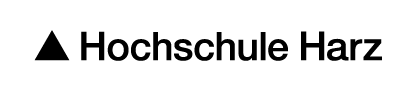
\includegraphics{hsh-logo-blank}}

\newcommand{\advisorone}{Prof.\ Axel Kaune}
\newcommand{\departmentone}{\ifgerman{\school}{\school}}

\newcommand{\advisortwo}{Prof.\ Thomas Leich}
\newcommand{\departmenttwo}{\ifgerman{\school}{\school}}

% Thesis kind
\ifgerman{\newcommand{\thesiskind}{Masterarbeit}}{\newcommand{\thesiskind}{Master's Thesis}}
%\ifgerman{\newcommand{\thesiskind}{Bachelorarbeit}}{\newcommand{\thesiskind}{Bachelor Thesis}}


\ifgerman{
	\newcommand{\theforename}{Niklas}
	\newcommand{\thesurname}{Kiefer}
	\newcommand{\thetitle}{Evaluation agiler Praktiken als Change Management Instrumente in der Digitalen Transformation}
	\newcommand{\thedate}{01. Juli 2019}
}{
	\newcommand{\theforename}{Niklas}
	\newcommand{\thesurname}{Kiefer}
	\newcommand{\thetitle}{Evaluation of Agile Practices as Change Management Instruments in Digital Transformation}
	\newcommand{\thedate}{July 1st, 2019}
}
\newcommand{\theyear}{2019}

%*********************************************************************%
% SETUP                                                               %
%*********************************************************************%

% meta informations of the document
\hypersetup{
 pdfauthor={\theforename\ \thesurname},
 pdftitle={\thetitle}
}

% open index file
\ifnotdraft{\makeindex}

%*********************************************************************%
% ACRONYMS                                                            %
%*********************************************************************%

% HOWTO: \gls{IDE} for singular or \glspl{IDE} for plural with 's
\newglossary[ch1]{formel}{ch2}{ch3}{Abkürzungsverzeichnis}
\makenoidxglossaries
\loadglsentries{glossaries/glossaries}
\glsaddall
%\glsaddall % use only if you have acronyms that occur only in graphics

%*********************************************************************%
% THE DOCUMENT                                                        %
%*********************************************************************%

\begin{document}

\ifgerman{
	\labelformat{lstlisting}{Quelltext~#1}
	\renewcommand{\lstlistingname}{Quelltext}
}{
	\labelformat{lstlisting}{Listing~#1}
}

% set the path where graphics are located
\graphicspath{{pics/}}

\ifnotdraft{
	\frontmatter
	\pagenumbering{roman}
	\newcommand{\theauthor}{\theforename\ \thesurname}
\newcommand{\theauthorr}{\thesurname,\ \theforename}
\begin{titlepage}
 \thispagestyle{empty}
 \begin{center}
  {\university}\\[0.4cm]
  {\school}\\[2.0cm]
   \hbox{}\hfill
    \begin{minipage}[t]{\textwidth}
      \begin{center}
      	\logo
      \end{center}
    \end{minipage} 
   \hfill\hbox{}
  \ \\[0.4cm]
  {\large \thesiskind \\[1cm]}
  {\huge\bf \thetitle \\[1cm]}
  { \ifgerman{Autor:}{Author:}}\\[0.4cm]
  {\huge \theauthor}\\[0.8cm]
  {\large\thedate}\\[0.8cm]
  {\ifgerman{Betreuer:}{Advisors:}}\\[0.4cm] 
  {\large
\advisorone
  }\\[0.2cm]
  {
\departmentone
  }\\[0.8cm]
  {\large
\advisortwo\ 
  }\\[0.2cm]
  {
\departmenttwo\ 
  }
 \end{center}
\end{titlepage}

%%%%%%%%%%%%%%%%%%%%%%%%%%%%%%%%%%%%%%%%%%%%%%%%%%%%%%%%%%%%%%%%%%%%%%%%%%%%
%%% Titelrückseite: Bibliographische Angaben
%%%%%%%%%%%%%%%%%%%%%%%%%%%%%%%%%%%%%%%%%%%%%%%%%%%%%%%%%%%%%%%%%%%%%%%%%%%%

\thispagestyle{empty}
\vspace*{\fill}
\begin{minipage}{15.0cm}
\textbf{\theauthorr:}\\
\emph{\thetitle\\}
\thesiskind, \university, \theyear.
\end{minipage}
\newpage

	\ifgerman{\chapter*{Inhaltsangabe}}{\chapter*{Abstract}}

Das Ziel einer jeden Digitalen Transformation ist eine Neuausrichtung von Unternehmen, um den Herausforderungen und Ansprüchen der gegenwärtigen Epoche der Digitalisierung gewachsen zu sein. Bei diesen großangelegten Veränderungen kann es gleichermaßen zu weiteren Herausforderungen und Problemen kommen, die mithilfe bestimmter Techniken begegnet werden können. Eine erfolgreiche Digitale Transformation ist notwendig, um dauerhaft konkurrenzfähig zu bleiben. 

Die vorliegende Arbeit untersucht mithilfe eines zweiteiligen systematischen Literaturreviews mögliche Problemfelder der Digitalen Transformation von Großunternehmen. Des Weiteren werden agile Methoden erarbeitet, die vermehrt Eingang in den Transformationsprozess gefunden haben. In einer anschließenden Evaluation werden beide Untersuchungsergebnisse miteinander verknüpft, indem weiter untersucht wird, in welchem Problembereichen die ausgewählten agilen Methoden einsetzbar sind.

Insgesamt wurden im ersten Review 23 Fallstudien systematisch untersucht, zusammengefasst und geclustert, wodurch sich 21 Problemfelder der Digitalen Transformation erarbeiten ließen. Im zweiten Review wurden 32 Fallstudien und Fachliteratur zu der Thematik untersucht, wodurch 18 agile Methoden extrahiert werden konnten. Diese wurden anschließend mittels eines klaren Schemas evaluiert.

Als Ergebnis werden eine Reihe von Leitlinien für eine erfolgreiche Anwendung von agilen Methoden in der Digitalen Transformation aufgestellt. Diese können als Ansatzpunkt für die Planung von Veränderungsprozessen im Kontext der Digitalen Transformation genutzt werden.


	\blankpage
}

%*********************************************************************%
% LISTINGS                                                            %
%*********************************************************************%

\ifnotdraft{
	{\parskip 0pt \pdfbookmark{\contentsname}{\contentsname}\chapterheadfont \tableofcontents} % toc bitte einzeilig
	\blankpage

	\ifgerman{
		\listoffigures
		\addcontentsline{toc}{chapter}{Abbildungsverzeichnis}
		
		\newpage

		\listoftables
		\addcontentsline{toc}{chapter}{Tabellenverzeichnis}
		
		\newpage

		\renewcommand*{\firstacronymfont}[1]{\emph{#1}}
		\printnoidxglossary[style=long,title=Abkürzungsverzeichnis,toctitle=Abkürzungsverzeichnis]
	}{
		\listoffigures
		\addcontentsline{toc}{chapter}{List of Figures}
		
		\newpage

		\listoftables
		\addcontentsline{toc}{chapter}{List of Tables}

		%\renewcommand*{\firstacronymfont}[1]{\emph{#1}}
		%\printglossary[type=acronym,title=List of Acronyms,toctitle=List of Acronyms]
	}
}

%*********************************************************************%
% CHAPTERS                                                            %
%*********************************************************************%

\mainmatter
\pagenumbering{arabic}

\chapter{Einführung}
\label{introduction}
%- Hintergrund
%- Motivation
%- Ziele
%- Aufgaben
%- Allgemeine Beschreibung des Projektes
%- Worum geht es in dieser Arbeit?
%- Wer hat die Arbeit veranlasst und wozu?
%- Wer soll von den Ergebnissen profitieren?
%- Welches Problem soll gelöst werden? Warum?
%- Unter welchen Umständen braucht man eine Verbesserung?
%- Was ist der Stand der Technik?
%- Welche noch offenen Probleme gibt es?
%- Worin unterscheidet sich mein Ansatz von den bisherigen?
%- Welche Ziele hat die Arbeit?
%- Wie will ich diese Ziele erreichen?
%- Was habe ich im Einzelnen vor?

\todo{Umformulierung?}
Die gegenwärtig stark einhergehende Digitalisierung des privaten, beruflichen und öffentlichen Lebens verändert die Art wie Unternehmen untereinander konkurrieren, Werte schaffen und mit ihren Geschäftspartnern und Kunden interagieren \cite[S. 1]{oswald_digitale_2018}.

Die sogenannte Digitale Transformation wird ein zunehmend wichtig werdender Veränderungsprozess, um die gegenwärtigen Potenziale neuer Innovationen wie Big Data, künstliche Intelligenz oder Cloud Computing konsequent auszunutzen und stetig Wettbewerbsvorteile zu generieren \cite[S. 2]{oswald_digitale_2018}. Klassische Führungskonzepte greifen nicht mehr, Stichworte wie Flexibilität, Schnelligkeit, Dynamik und Kundenorientierung sind essentielle Voraussetzungen. 

Das Aufbrechen alteingesessener Strukturen bis hin zur Transformation zu einem digitalen Unternehmen bringt jedoch hohe Probleme mit sich. Bei einer erfolgreichen Umsetzung des Veränderungsprozesses spielen eine große Reihe von Einflüssen mit ein. Oft bremsen gerade alte Strukturen den Erfolg der Veränderungen, was gerade bei der Forderung nach Flexibilität und Dynamik ein großes Problem darstellt
\cite[S. 196]{appelfeller_digitale_2018}


Sogenannte agile Methoden können helfen, Probleme des klassischen Change Managements in der Digitalen Transformation zu bearbeiten. Praktiken wie z.B. Design-Thinking oder DevOps haben sich bereits als Projektmanagement-Instrumente bewährt \cite[S. 7]{deeken_agiles_2018}. Interessant ist jedoch auch die Herangehensweise, sie im größeren Umfeld einer Organisationskultur einzusetzen, um mithilfe der Bildung einer Agilen Kultur den Transformationsprozess zu optimieren \cite[S. 140]{hofert_agiler_2016}.

Im Folgenden soll auf den genauen Forschungsschwerpunkt der vorliegenden Arbeit eingegangen werden. Es wird eine Einführung über Problematiken innerhalb der Digitalen Transformation gegeben und die exakte Zielstellung der Arbeit aufgeführt. Außerdem wird nachfolgend der Aufbau der Arbeit geklärt und erläutert, mithilfe welcher Methodik die aufgeführten Fragestellungen beantwortet werden sollen.

\section{Problemstellung}

\todo{Grafik einer Studie einbauen?}

''Die Diskussion rund um digitale Transformation ist geprägt von Hypes und dringenden Warnungen, die zum Handeln anregen sollen.'' \cite[S. 12]{berghaus_2016}. Innerhalb der Digitalisierung kommt es zu einem zunehmenden Druck um die Aufrechterhaltung eines konkurrenzfähigen Geschäftsmodells. Das Aufkommen immer neuer Innovationen in verschiedenen Technologien bildet zudem eine Gefährdung durch neue Möglichkeiten von Markteintritten, bis hin zur Zerschlagung altbewährter Geschäftsmodelle, sogenannte Digitalen Disruptionen \cite{urbach_digitalization_2018}.

Diese Gefährdungen treiben Großunternehmen dazu, gegenwärtige Strukturen zu überdenken und Veränderungen einzuleiten. \todo{Zitat finden!} Vornehmlich die Digitalisierung des Geschäftsmodells, aber auch der gesamten Unternehmensstruktur samt - kultur sind wichtige Themen in den Führungsebenen großer, internationaler Unternehmen \cite[S. 18]{buhse_transformationswerk_2016}. Das Bestreben nach Veränderungen hin zu einem digitalen Unternehmen ist also erkennbar in den Köpfen von Management und Führung. Trotzdem lassen Studien wie von \citeA{buhse_transformationswerk_2016} erkennen, dass solch ein großangelegter Veränderungsprozess wie die Digitale Transformation ebenso große Problemfelder mit sich bringen kann. Oft mangelt es schon an erfolgreicher Kommunikation innerhalb des Unternehmen, beispielsweise hervorgerufen durch ''existente Vernetzungslücken und Defizite in der internen Kommunikation'' \cite[S. 18]{buhse_transformationswerk_2016}.

Zur Bekämpfung klassischer Probleme in großen Veränderungsprozessen bedarf es oft externer Hilfe. Promotoren oder Inkubatoren können helfen, Problemfelder im Transformationsprozess anzugehen \todo{Zitat Kaune Buch?}. \citeauthor{zillmann_status_2017} geht in seiner Studie sogar soweit, dass ''$\lbrack$o$\rbrack$hne externe Beratungs- und IT-Dienstleister $\lbrack$...$\rbrack$ all diese Herausforderungen nicht zu bewältigen'' (S. 16) wären. Interne Treiber können aber ebenfalls dazu beitragen, solche Problemfelder anzugehen. Oft fehlt es allein schon an kulturellen Veränderungen innerhalb des Unternehmens \cite{hofert_agiler_2016} \todo{Seite?}. Ein sogenanntes ''Agiles Mindset'' kann helfen, einen  solchen ''Kulturwandel'' einzuleiten \cite{hofert_agile_2018}.

Eine wesentliche Fragestellung der vorliegenden Arbeit soll es sein, eine Reihe solcher Problemfeldern zu identifizieren, die eine angestrebte Digitale Transformation gefährden. Daraus resultierend soll untersucht werden, inwieweit der Einsatz sogenannter Agiler Praktiken diese lösen können.

\section{Forschungsfragen und Zielstellung}

Die zu erstellende Arbeit soll sich mit folgenden grundlegenden
Fragestellungen beschäftigen:

\begin{itemize}[noitemsep, topsep=0pt]
	\item \textit{FS1}: Wie sehen allgemeine Veränderungsprozesse im Zuge der Digitalen Transformation aus?
	\item \textit{FS2}: Welche Probleme treten bei der Digitalen Transformation eines Großunternehmens auf?
	\item \textit{FS3}: Welche agilen Praktiken haben sich in großen Organisationen innerhalb des Transformationsprozesses etabliert?
	\item \textit{FS4}: Wie können agile Methoden dazu beitragen, die vorher erarbeiteten Probleme zu heben?
	\item \textit{FS5}: Welche Handlungsmuster lassen sich für einen erfolgreichen Einsatz agiler Praktiken im Transformationsprozess ableiten (Best Practices)?
\end{itemize}
Der erste Schwerpunkt besteht in der Extraktion verschiedener Veränderungsprozesse innerhalb des Transformationsprozesses von Großunternehmen (vgl. FS1). Zu erfassende Veränderungsmuster sind bestimmte Komponenten, die von der Digitalen Transformation direkt betroffen sind. Dies können beispielsweise unternehmensinterne Strukturen, aber auch das Geschäftsmodell des Unternehmens. Grundsätzlich sollen folgende Fragen beantwortet werden: Was \textit{verändert} sich im Unternehmen? Was soll genau \textit{digitalisiert} werden? Anschließend soll weiterhin erschlossen werden,  in welchen Bereichen es zu Problemen im Veränderungsprozess kommen kann (vgl. FS2).

Der zweite große inhaltliche Schwerpunkt ist der Einsatz agiler Praktiken im Transformationsprozess. Es soll untersucht werden, welche Praktiken derzeit in der Digitalen Transformation angewendet werden (vgl. FS3). Es soll somit eine Art \textit{Status Quo} geschaffen werden, um die Relevanz agiler Praktiken besser einschätzen zu können. Anschließend soll sich eine Bewertung eben dieser agilen Methoden vorgenommen werden (vgl. FS4). Als Ergebnis dessen soll die vorliegende Arbeit mögliche Best Practices für den Einsatz agiler Praktiken im Transformationsprozess erarbeiten (vgl. FS5). Dadurch kann ein Anreiz geschaffen werden, solche Methoden gezielt im Veränderungsmanagement einzusetzen. 

Die konkrete Zielstellung besteht darin, agile Praktiken hinsichtlich ihrer Anwendbarkeit bei Problemen innerhalb des Digitalen Transformation von Großunternehmen zu evaluieren. Der genaue Aufbau dieses Vorhabens wird in den folgenden Abschnitten beschrieben (vgl. \ref{introduction:schema} und \ref{introduction:methods}).

\section{Aufbau der Arbeit}
\label{introduction:schema}

Zur Orientierung der Vorgehensweise zur vorliegenden Arbeit soll ein kurzer Überblick über den Aufbau gegeben werden. Abbildung \ref{fig:aufbau} skizziert das wesentliche Schema.

\begin{figure}
	\centering
	\fbox{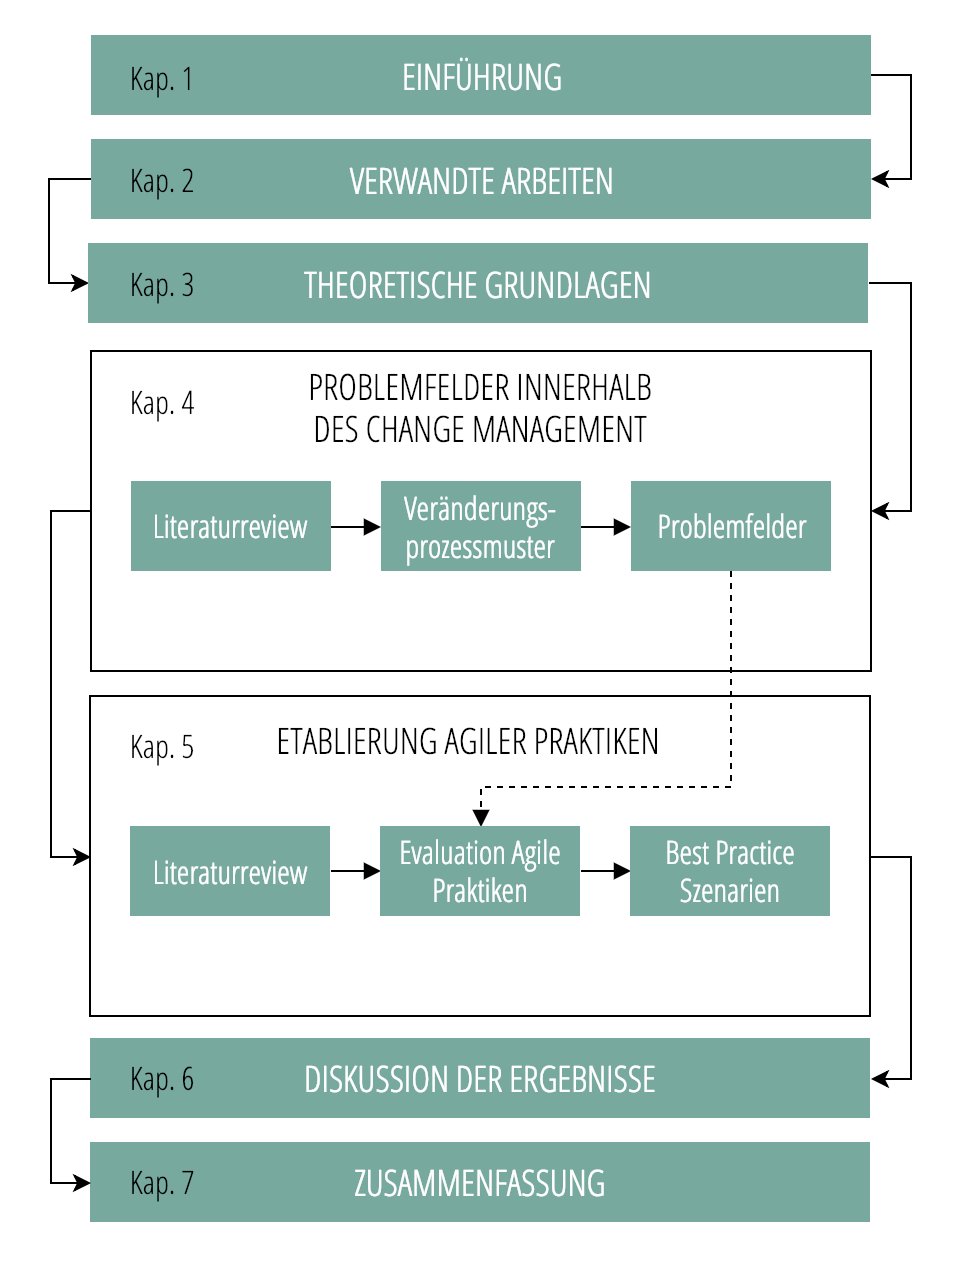
\includegraphics[width=0.5\linewidth]{pics/aufbau}}
	\caption[Aufbauschema der Arbeit]{Aufbauschema der Arbeit (eigene Darstellung)}
	\label{fig:aufbau}
\end{figure}

Aufbauend auf die Einführung in die wesentliche Problematik  (vgl. \ref{introduction}) wird anschließend ein Überblick über artverwandte Arbeiten in dem Thema aufgeführt (vgl. \ref{relatedwork}). Es wird erläutert, welcher Forschungsstand im wesentlichen bereits vorliegt und wir sich die vorliegende Arbeit abgrenzt. Zum Aufbau eines besseren Verständnisses innerhalb der Thematik schließt der einleitende Teil mit einer theoretischen Einführung in wichtige Komponenten (vgl. \ref{background}). In diesem Abschnitt werden zudem wichtige Begriffsabgrenzungen vorgenommen.

Der Hauptteil der Arbeit gliedert sich in zwei wesentliche Abschnitte. Zunächst werden in \ref{problemfields} mithilfe eines Literaturreviews relevante Veränderungsprozessmuster und Problemfelder innerhalb der Digitalen Transformation in Großunternehmen erarbeitet. Anschließend werden weiterhin durch ein zweites Literaturreview eine Reihe von genutzten Agilen Praktiken im Transformationsprozess zusammengestellt, welche anschließend nach einem genauem Schema evaluiert werden (vgl. \ref{agilepractices}). Auf dieser Grundlage werden im Kapitel abschließend Best Practice Szenarien für den Einsatz agiler Praktiken im Transformationsprozess aufgestellt. Der Zusammenhang beider Hauptteile wird im nachfolgenden \ref{introduction:methods} erklärt.

Die Ergebnisse aus den vorhergehenden Abschnitten werden in \ref{evaluation} kritisch diskutiert. Abschließend wird eine Zusammenfassung über die Erkenntnisse der vorangestellten Untersuchungen aufgeführt (vgl. \ref{conclusion}).


\section{Methodisches Vorgehen}
\label{introduction:methods}

% - allgemeines Vorgehen, mit Verweis auf die methodischen Unterkapitel der einzelnen Abschnitte. Systematischer Literaturreview + Metastudie als spezielle Form, Evaluation am Ende der zweiten Metastudie

Das übergeordnete Ziel soll die Evaluation agiler Praktiken im Kontext der Digitalen Transformation sein. Dafür soll zunächst ein systematischer Literaturreview vorgenommen werden. Dieses Review wird in zwei großen Bestandteilen durchgeführt. Zunächst soll in \ref{problemfields} eine Reihe von Fallstudien systematisch analysiert werden. Eine weiteres, methodisch vom ersten getrenntes  Review wird dann in \ref{agilepractices} vorgenommen. Beide Systematischen Literaturreviews haben das Wesen einer Metastudie, da vornehmlich Erkenntnisse getätigter Fallstudien im Bereich der Digitalen Transformation ausgewertet und zusammengefasst werden  \todo{in Fußnote erklären oder Zitat?}. Allgemeine Fachliteratur wird in beiden Fällen keine große Bedeutung zuteil, mit einer kleinen Ausnahme innerhalb des zweiten Reviews in \ref{agilepractices}. Die genaue Vorgehensweise, sowie Ein - und Ausschlusskriterien werden in den jeweiligen Abschnitten zum Methodischen Vorgehen noch erläutert (vgl. \ref{problemfields:methods} und \ref{agilepractices:methods}).

Das Ziel der zweigeteilten Literaturreviews soll es sein, relevante Ergebnisse aus bereits getätigten Studien und Fallstudien zu analysieren und zusammenzufassen, um sie für die nachfolgende Evaluation gezielt einsetzen zu können. Mithilfe der Analyse verschiedenster aktueller Studien und Fallstudien soll ein möglichst gegenwärtiges Bild der Situation in internationalen Großunternehmen dargestellt werden.

Als weiterer methodischer Schwerpunkt in der vorliegenden Arbeit wird eine Evaluation vorgenommen. Diese dient in \ref{agilepractices} dazu, die mithilfe des Literaturreviews erarbeiteten agilen Praktiken in Bezug auf Anwendbarkeit in bestimmten Problemfeldern (vgl. \ref{problemfields}) zu bewerten. Die Evaluation wird nach einem klaren Bewertungsschema vorgenommen. Das Schema und die Bewertungskriterien werden im dazugehörigen methodischen \ref{agilepractices:methods} dargestellt.

\todo{noch erweitern?}

\chapter{Verwandte Arbeiten}
\label{relatedwork}

% - Übersicht über artverwandte Arbeiten zum gleichen Thema
% - Wichtig: Herausarbeitung über thematische Einordnung der eigenen Leistung
% - + Darstellung über Mehrwert

Ein wesentlicher Schwerpunkt der vorliegenden Arbeit ist eine  Untersuchung von agilen Methoden als Einflussfaktor in der Digitalen Transformation. Durch die hohe Aktualität der Digitalen Transformation ist der Forschungsstand als relativ neuartig anzusehen. Trotzdem gibt es bereits eine Reihe veröffentlichter Publikationen, die sich mit einer ähnlichen Thematik beschäftigen. Diese sollen nachfolgend kurz vorgestellt und darüber hinaus der Beitrag der vorliegenden Arbeit hervorgehoben werden.

\shortciteA{vuksic_preliminary_2018} nahmen in ihrer Arbeit ein systematisches Literaturreview zur Digitalen Transformation vor. Sie stellen dar, dass der aktuelle Forschungsstand in diesem Bereich derzeit noch sehr unerforscht sei. Eins ihrer vordergründigen Erkenntnisse ist es, dass der Transformationsprozess sowohl das stetige Aufnehmen neuer Technologien in das eigene Geschäftsmodell, als auch interne organisationale Veränderungen bedingt (S. 1). Sie fanden heraus, dass neuartige Change Management Instrumente nötig seien, um den Herausforderungen der Digitalen Transformation zu begegnen.

Ein weiteres systematisches Literaturreview nahmen \shortciteA{dikert_challenges_2016} vor. Sie fassen detailliert zusammen, welche Herausforderungen und Erfolgsfaktoren in einer Agilen Transformation zu finden sind. Dabei wird ein starker Bezug auf die Anwendungen verschiedener agiler Methoden gelegt (S. 1).  Einen ähnlichen Ansatz verfolgen \shortciteA{osmundsen_digital_2018}. Methodisch wurde ebenfalls ein SLR gewählt, als Ergebnis werden Erfolgsfaktoren und Problemfelder der Digitalen Transformationen vorgestellt. Es wird vermehrt dargestellt, welchen Einfluss die Transformation auch auf die Organisation des Unternehmens hat (S. 1).

Einen direkten Bezug zwischen agilen Methoden und weitreichenden organisationalen Veränderungen beschriebt \citeA{hofert_agiler_2016} in ihrer Arbeit. Es wird deutlich, welche Möglichkeiten Führungskräfte aktuell haben, um Problemen für großangelegte Veränderungen zu begegnen, wie beispielsweise die Digitalisierung. Dafür werden eine Reihe agiler Methoden aufgeführt und erklärt, wie anhand dieser ein neuer Führungsstil implementiert werden kann.

\citeA{weinreich_lean_2016} legt den Kern seines Buches zu Lean Digitization ebenfalls auf eine Verbindung zwischen agilen Methoden und großen Veränderungen in Unternehmen. Es gibt einen klaren Bezug zur Digitalen Transformation. Es werden explizite Erfolgsfaktoren für den Einsatz agiler Methoden im Transformationsprozess genannt, beispielsweise für Design Thinking (S. 19f.). 

Die vorliegende Arbeit versucht ebenfalls eine Verbindung zwischen agilen Methoden und der Digitalen Transformation zu schaffen. Aufbauend auf den Einsatz eines mehrschichtigen SLR sollen explizite Veränderungsmuster und Problemfelder des Transformationsprozesses ermittelt werden. Daran anschließend werden agile Methoden hinsichtlich ihrer Einsetzbarkeit bei diesen Problemen untersucht. Der vordergründige Beitrag soll es sein, Muster für einen erfolgreichen Einsatz agiler Methoden zu finden. Inhaltlich kommt dies den Ergebnissen von \citeA{weinreich_lean_2016} nahe. Darüber hinaus verfolgt die vorliegende Arbeit einen sehr systematischen Einsatz, in dem eine ganze Reihe agiler Methoden untersucht werden. Es soll ein Überblick über Problemfelder und mögliche Lösungsansätze der Digitalen Transformation geschaffen werden, was Anreize für nachfolgende, spezifischere Untersuchungen schafft.

\chapter{Theoretische Grundlagen}
\label{background}

%- Allgemeine Wissensgrundlagen des Fachgebiets
%- Spezielle Grundlagen, die für das Verständnis erforderlich sind
%- Rahmenbedingungen für die Arbeit
%- Ausführungen zum Stand des Wissens / der Technik
%Als Leitprinzip gilt: Nur Informationen erwähnen, die
%- später benötigt werden,
%- notwendig sind, um die Arbeit oder ihre Motivation zu verstehen
%Das heißt insbesondere,
%- keine Inhalte aus Lehrbüchern, außer
%- diese werden benötigt, um Problemstellung oder Lösungsweg zu definieren.

Ziel des nachfolgenden Kapitels soll es sein, eine allgemeine Wissensgrundlage über wesentliche Begrifflichkeiten im Thema zu schaffen. Um die nachfolgenden Ausführungen im Hauptteil (vgl. \ref{problemfields} und \ref{agilepractices}) besser nachvollziehen zu können, sollen wichtige Definitionen und Begriffsabgrenzungen vorgenommen werden.

\section{Digitale Transformation}
\label{background:dt}

Der wesentliche Schwerpunkt der vorliegenden Arbeit dreht sich um die sogenannte \textit{Digitale Transformation}. Eine allgemeine Definition für diese Begrifflichkeit ist momentan schwer zu finden \cite[S. 3]{schallmo_digitale_2017}. Grundsätzlich versteht man unter der Digitalen Transformation von Unternehmen den Einfluss neuer Technologien und Innovationen auf gesamtunternehmerische Strukturen, Geschäftsmodelle und Wertschöpfungsketten \cite{oswald_digitale_2018}. Nach \citeA{kofler_digitale_2018} sei es das Ziel der digitalen Transformation, Unternehmen fortlaufend und ohne vorhersehbares Ende so umzubauen, dass sie sich den kontinuierlichen Marktveränderungen durch Digitalisierung stellen können (S. 1). Man erkennt hierbei das Muster, dass die Begrifflichkeit der \textit{Digitalisierung} ein wichtiger Faktor für den strategischen Aufbau von Unternehmen geworden ist. Neue Innovationen im digitalen Bereich machen es vor allem kleineren Firmen einfacher in bestehende Märkte einzutreten und sogenannte \textit{Disruptionen} \todo{Erklärung als Fußnote} zu erschaffen. 
 
 
 Viele Versuche einer Definition betreffen immer den Bezug auf aufkommende digitale Technologien. Diese können als sogenannte \textit{Treiber} der Digitalen Transformation bezeichnet werden \cite[S.20]{bloching_digitale_2015}. \ref{fig:bigpicture} skizziert eine Übersicht dieser verschiedenen Treiber. Man erkennt hierbei schon wichtige Handlungsfelder des Transformationsprozess, wie beispielsweise die Automatisierung von Geschäftsprozessen oder die Nutzung von generierten Digitalen Daten. Solche Handlungsfelder werden in der vorliegenden Arbeit in \ref{problemfields:changepatterns} genauer erläutert.
 
\ref{fig:bigpicture} kennzeichnet außerdem, dass eine große Reihe von neuen Technologien die Digitale Transformation antreiben. Beispielsweise bilden Technologien wie \textit{Cloud Computing} oder \textit{Big Data} neue Möglichkeiten für digitalisierte Geschäftsmodelle. 
 
\begin{figure}[H]
	\centering
	\fbox{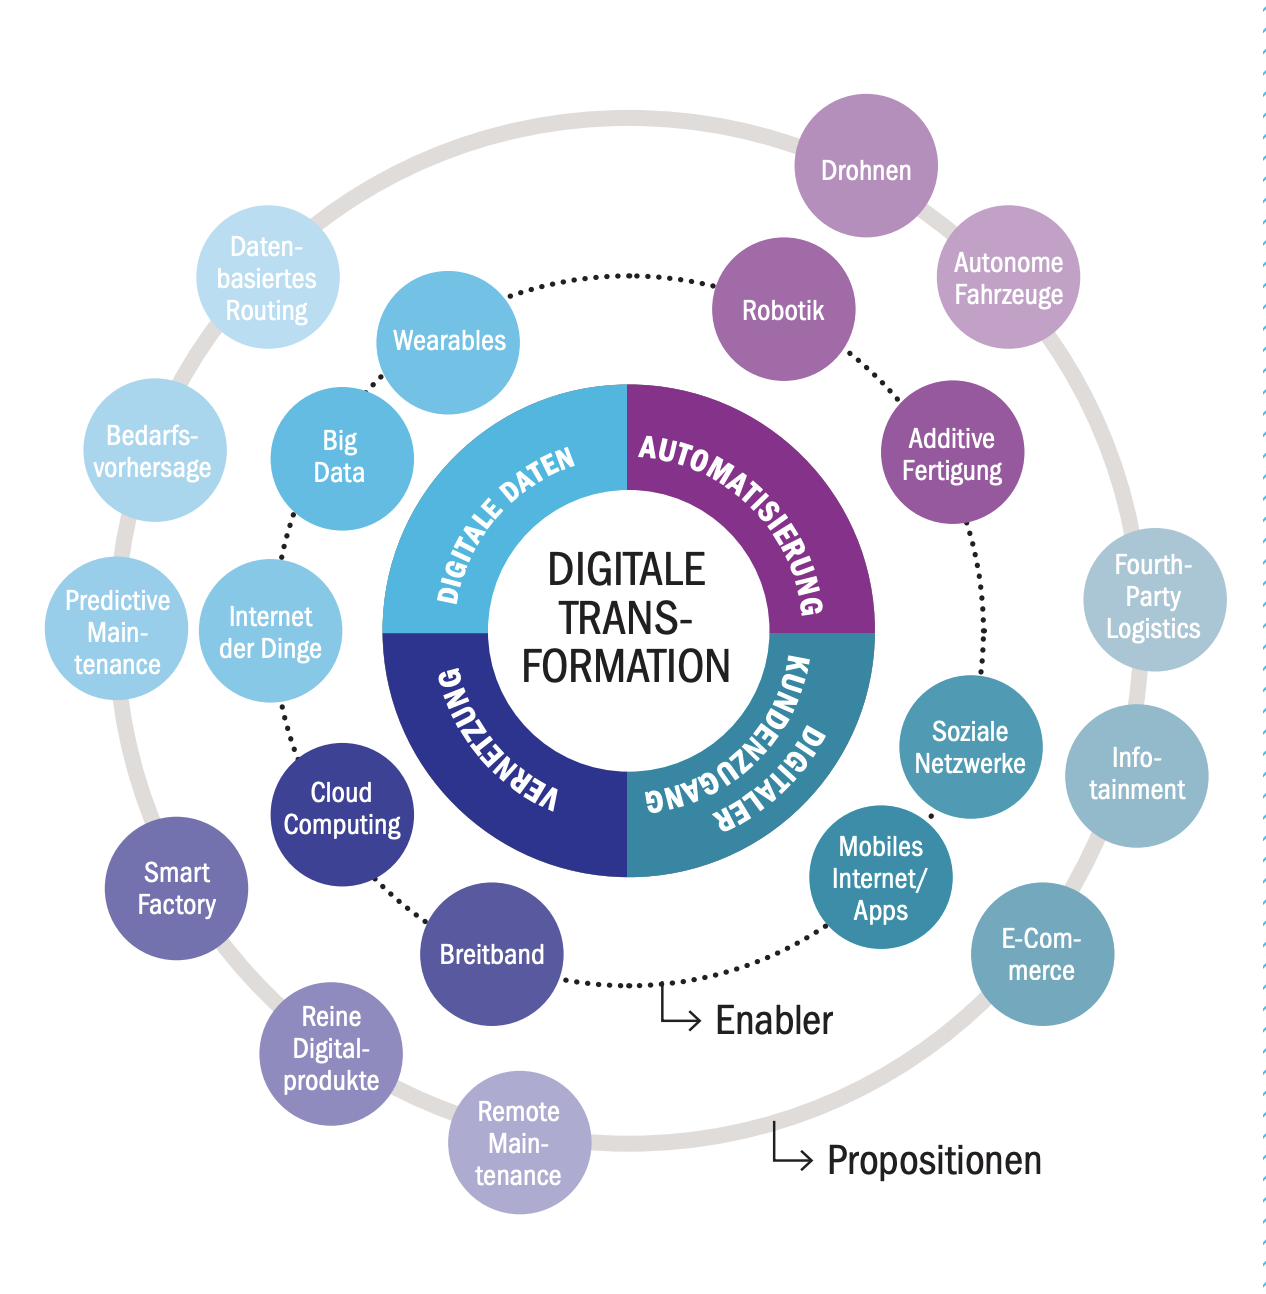
\includegraphics[width=0.7\linewidth]{pics/dtbigpicture}}
	\caption[Big-Picture der Digitalen Transformation]{Treiber der Digitalen Transformation \protect \cite[S. 20]{bloching_digitale_2015}}
	\label{fig:bigpicture}
\end{figure}

Die Digitale Transformation kann somit als weitreichender Veränderungsprozess von Unternehmen angesehen werden. \citeA{oswald_digitale_2018} beschreiben innerhalb dieses Prozesses vier bestimmende Charakteristika. Demnach sei die Digitale Transformation ''unausweislich, unumkehrbar, ungeheuer schnell und mit Unsicherheit behaftet`` (S. 10). Man erkennt hierbei also ein gewisses Risiko bei der Bearbeitung einer solchen Transformation. Es ginge für das Unternehmen vor allem darum, ''die Chancen neuer, digitaler Technologien kontinuierlich hinsichtlich ihres Potentials zur Weiterentwicklung bestehender Geschäftsmodelle zu evaluieren`` (S. 10).

Es kristallisiert sich ganz klar heraus, dass der Veränderungsprozess einer Digitalen Transformation zwar unausweichlich ist, um die eigene Marktposition zu verteidigen. Trotzdem zeigen sich zunehmende Risiken und Probleme bei der Implementierung solcher Veränderungen. Demnach liegt es nahe, sich in der vorliegenden Arbeit mit den Problemfeldern der Digitalen Transformation zu beschäftigen (vgl. \ref{problemfields}).

\section{Change Management}

\begin{figure}[h]
	\centering
	\fbox{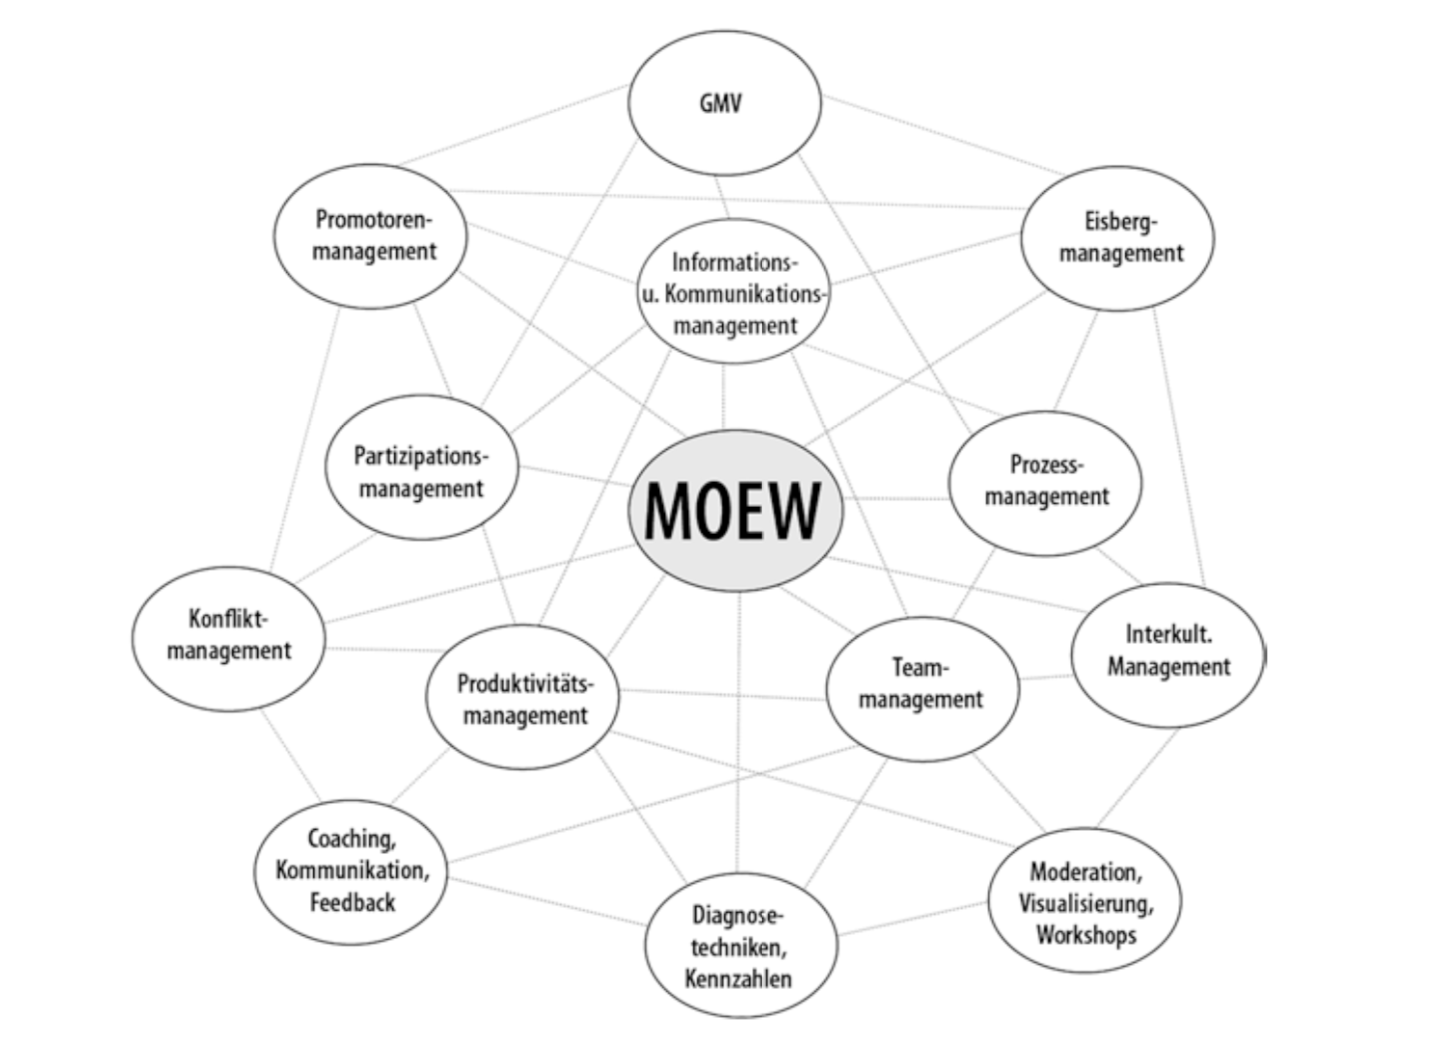
\includegraphics[width=0.7\linewidth]{pics/moew}}
	\caption[Bestandteile des MOEW-Modells]{Bestandteile des MOEW-Modells \protect \cite[S. 12]{kaune_change_2016}}
	\label{fig:moew}
\end{figure}
\todo{eventuell Bild verbessern}

Wie im vorhergehenden Abschnitt bereits angeklungen ist, handelt es sich bei der Digitalen Transformation um einen großangelegten Veränderungsprozess eines Unternehmens. Vordergründig kann definiert werden, dass es sich beim Veränderungsmanagement bzw. \textit{Change Management} um das ''$\lbrack$m$\rbrack$anagen von Veränderungen in Unternehmen und Organisationen`` \cite[S. 10]{kaune_change_2016} handelt. Durch die gravierenden Änderungen des Unternehmens und die Notwendigkeit, einen geordneten Veränderungsprozess anzustoßen, kann das Steuern der Digitale Transformation grundsätzlich als Change Management bezeichnet werden. Die Transformation muss gezielt gesteuert werden, eine eigenes Management-Konzept ist unabdingbar um den Herausforderungen entgegenzuwirken \cite[S. 19]{hess_digitale_2019}. Nachfolgend sollen in kurzer Form verschiedene Change-Management-Ansätze gezeigt werden, um ein generelles Verständnis über diese Problematik zu erhalten.

Eine generelle Definition für die Begrifflichkeit konnte in den vorangestellten Ausführungen bereits aufgestellt werden \cite{kaune_change_2016}. Grundsätzlich können Veränderungsprozesse \textit{top-down} (z.B. Business Reengineering), d.h. revolutionär, von der oberen Managementabteilung zentral voran geführt; oder \textit{bottom-up} (z.B. Organisationsentwicklung), d.h. evolutionär, die Mitarbeiter stark einbindend; geprägt sein \cite[S. 10]{kaune_change_2016}. Soll eine Veränderung ''sozial und ökonomisch nachhaltig wirksam sein``, so \citeA{kaune_change_2016}, sei eher der zweite Ansatz zu wählen, da ''über
das Einbeziehen und die aktive Einbindung der Mitarbeiter Identifikation mit dem Veränderungsobjekt geschaffen wird`` (S. 11). Wie in \ref{background:dt} bereits angeklungen, dass eine kontinuierliche Lösung innerhalb der Digitalen Transformation Vorteile haben kann. Allerdings spricht man bei den vorzunehmenden Veränderungen von ''ungeheuer schnell``  \cite[S. 10]{oswald_digitale_2018} , so dass ebenfalls revolutionäre Ansätze einzusetzen wären. Ob und inwieweit die genannten Ansätze Einklang in einen Change-Management-Prozess für die Digitale Transformation von Großunternehmen finden, soll im weiteren Verlauf dieser Arbeit geklärt werden.

Als ein wesentlicher Punkt des Change Management innerhalb einer Digitalen Transformation wird die Einbeziehung der Mitarbeiter des Unternehmens genannt \cite[S. 179f.]{hess_digitale_2019}. \citeA{kaune_change_2016} beschreiben in ihren Ausführungen das sogenannte \textit{MOEW-Modell} (Moderne Organisationsentwicklung) als ein Ansatz der partizipativen Organisationsentwicklung (S. 11). Ohne zu genau auf die einzelnen Bestandteile einzugehen, zielt das Modell auf eine ''gleichzeitigen Verbesserung der Leistungsfähigkeit der Organisation und der Qualität des Arbeitslebens`` (S. 11) ab. Dabei werden verschiedenste Komponenten des Veränderungsmanagement, beispielsweise Partizipations-, Prozess- oder Kommunikationsmanagement, sowie eine Reihe von Tools und Techniken eng miteinander verknüpft werden, um Mitarbeiter direkt in den Veränderungsprozess mit einzubinden und einen langfristigen Erfolg zu erzielen (S. 11f.). \ref{fig:moew} zeigt die einzelnen Bestandteile des MOEW-Modells.

Die Einbindung und Beurteilung der Mitarbeiter des Unternehmens hat eine große Bedeutung im Veränderungsprozess inne. Den Menschen in den Mittelpunkt zu stellen ist ein wichtiges Erfolgskriterium, da jede Veränderung zwangsläufig immer den Menschen direkt betreffen \cite[S. 3]{bertagnolli_change_2018}. \ref{fig:changekurve} illustriert die sogenannte \textit{Change-Kurve} und gibt einen Überblick darüber, inwieweit sich das Verhalten von Mitarbeitern in einem Change-Management-Prozess verändert. ''Werden Menschen in Veränderungen nicht aktiv eingebunden oder nicht beachtet, wird der auftretende Widerstand noch stärker und letztendlich zu einer Blockade``, so \citeA{bertagnolli_change_2018} (S. 3f.). Ziel eines jeden Veränderungsprozesses solle es sein, Widerstand zu bearbeiten und möglichst zu beseitigen (ebenda). 

 \begin{figure}
	\centering
	\fbox{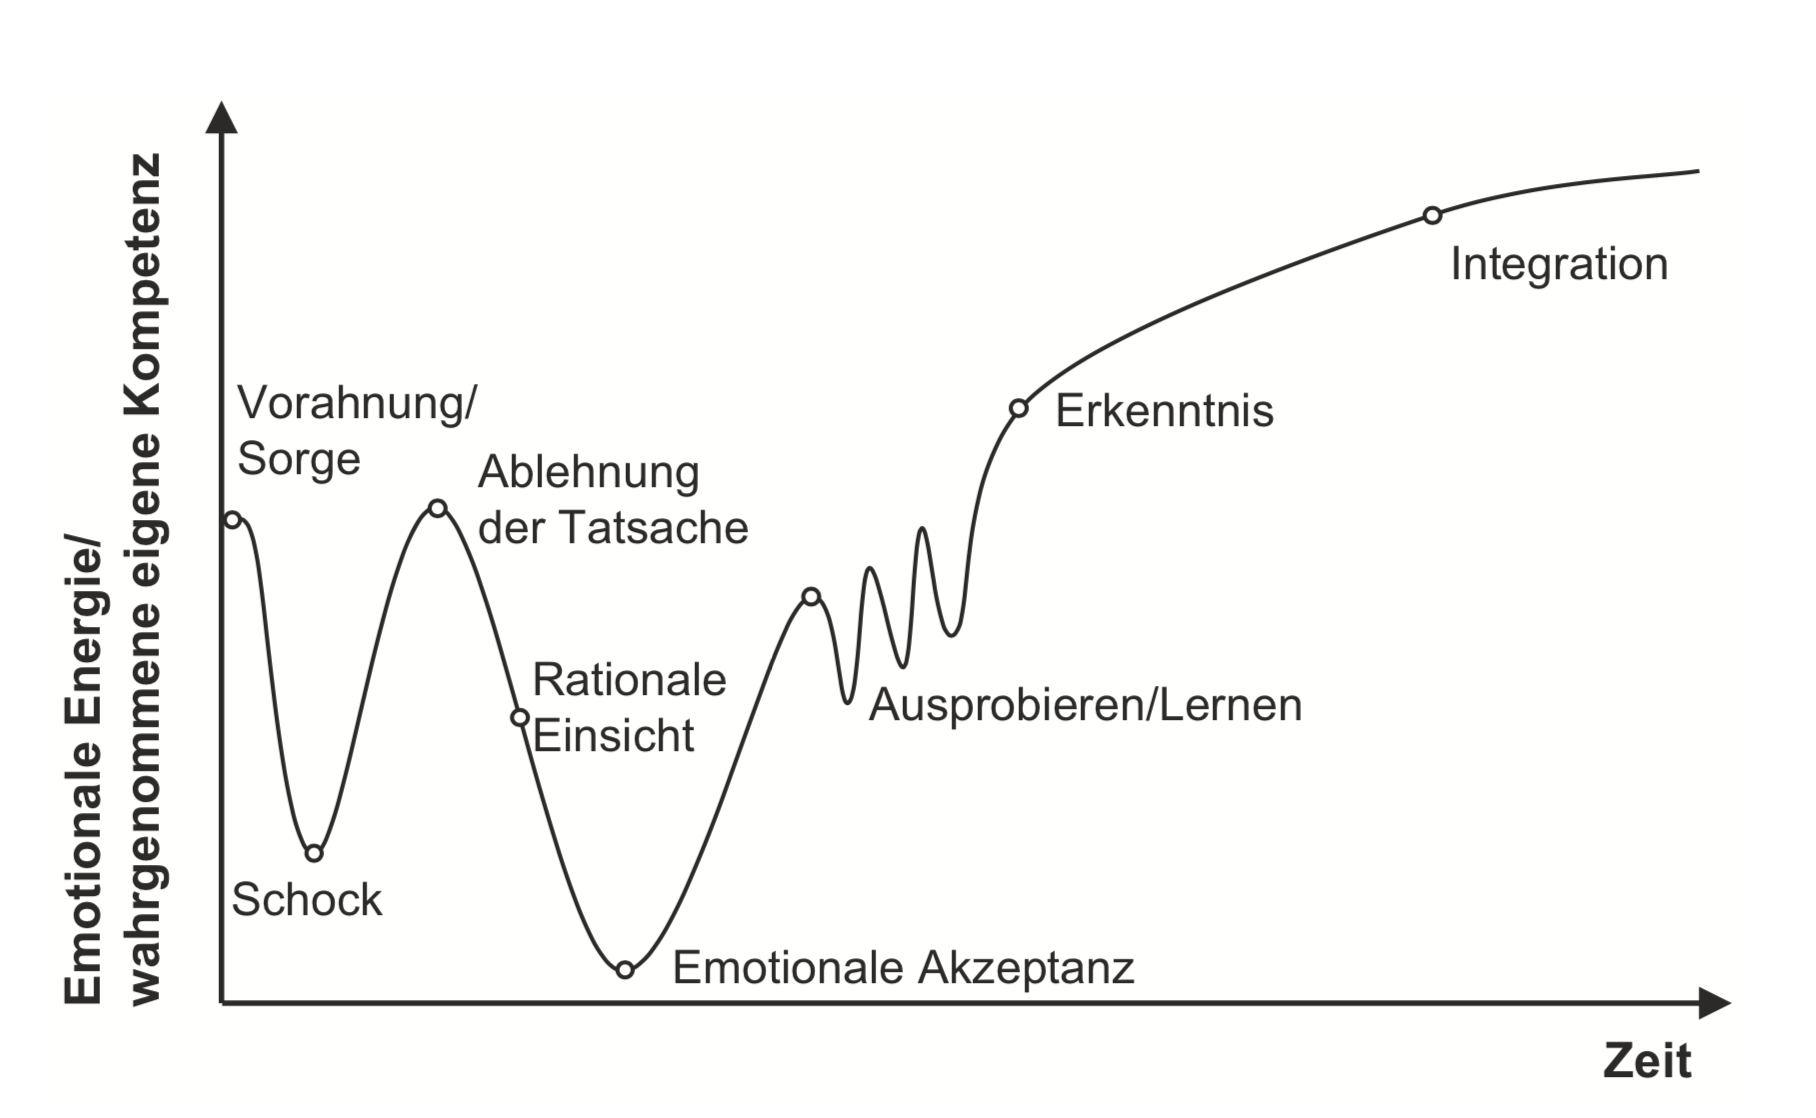
\includegraphics[width=0.8\linewidth]{pics/changekurve}}
	\caption[Change-Kurve von Mitarbeiterverhalten]{''Change-Kurve``: Veränderungsverhalten von Mitarbeitern \protect \cite[S. 3]{bertagnolli_change_2018}}
	\label{fig:changekurve}
\end{figure}

Neben den einzelnen Komponenten des Change Managements finden außerdem ausgewählte Werkzeuge Eingang in den Veränderungsprozess. Das genannte MOEW-Modell führt erste Beispiele auf, wie beispielsweise Coaching und Workshops. Neben diesen finden aber auch andere Techniken weite Anwendung. Ohne dem nächsten \ref{background:agile} etwas vorwegzunehmen, können hier Agile Methoden genannt werden, welche ebenfalls einen wesentlichen Schwerpunkt der vorliegenden Arbeit bilden. Gerade im Hinblick auf die Einbindung von Mitarbeitern erfreuen sich solche Praktiken großer Beliebtheit. Nach \citeA{olbert_uberlebenselixier_2019} sei es wichtig, ''Betroffene zu Beteiligten [zu] machen``, um damit zu erreichen, ''dass die vom Wandel Betroffenen nicht Objekte von Top-down-Entscheidungen, sondern Mitgestalter des
Wandels sind`` (S. 6). 

Die Verbindung der Agilität mit Change Management macht aus diesen Gesichtspunkten also durchaus Sinn. Deswegen erscheint für die vorliegende Arbeit die Einwirkung von Agilen Methoden in den Transformationsprozess als ein interessantes Untersuchungsgegenstand. Aus diesem Grund soll im folgenden ein kleiner Umriss über das Thema der Agilität gegeben werden.

\section{Agilität}
\label{background:agile}

Der Begriff  \textit{Agilität} in dem Kontext wie er in der vorliegenden Arbeit thematisiert wird liegt der Agilen Softwareentwicklung zu Grunde. Begründet wurde diese grundlegend im Jahre 2001 von einer Reihe erfahrener Softwareentwickler im sogenannten \textit{Agilen Manifesto} \cite{beck_manifesto}. Diese legten in eben diesem zudem vier wichtige Leitlinien der Agilen Softwareentwicklung fest (übersetzt aus dem Original):

\begin{itemize}[noitemsep, topsep=0pt]
	\item Individuen und Interaktionen stehen über Prozessen und Werkzeugen
	\item Funktionierende Software steht über einer umfassenden Dokumentation
	\item Zusammenarbeit mit dem Kunden steht über der Vertragsverhandlung
	\item Reagieren auf Veränderung steht über dem Befolgen eines Plans
\end{itemize}

Man erkennt hierbei sehr gut, dass ein wesentlicher Bestandteil Flexibilität und Reaktionsfähigkeit auf Veränderungen sind. Wichtige Fähigkeiten im Bezug der Digitalen Transformation \todo{Zitat?} Diese Prinzipien der Agilen Softwareentwicklung lassen sich ebenfalls auf größere Organisationen ausweiten. Nach \citeA{hofert_agiler_2016} ist ''Agilität [...] die Fähigkeit von Teams und Organisationen, in einem unsicheren, sich veränderndem und dynamischen Umfeld flexibel, anpassungsfähig und schnell zu agieren.`` (S. 5). Auf den genauen Begriff der \textit{Agilen Organisation} wird im  folgenden \ref{background:agileorganisation} noch eingegangen. Zunächst sollen weitere Schwerpunkte der Agilität definiert werden.

Neben den bereits aufgeführten agilen Leitlinien sind außerdem sogenannte \textit{Agile Werte}, \textit{Prinzipien} und \textit{Methoden}. Letzteres soll im folgenden nicht weiter ausgeführt werden, da Agile Methoden noch in \ref{agilepractices} detailliert aufgeführt werden. Zu erwähnen sei zunächst nur, dass solche als ``gebündelte Handlungen und in Konzepte übersetzte Aktionen, die auf den agilen Prinzipien beruhend oder in einem anderen Kontext entwickelt wurden, aber zum agilen Denken passen'' \cite[S. 17]{hofert_agiler_2016}.

Agile Werte gehören deshalb zu einem jeden erfolgreichen, agilen Prozess, weil sie die Haltung eines jeden Beteiligten direkt beeinflussen. Sie sorgen indirekt dafür, dass sich Mitarbeiter für ein Vorhaben besonders motivieren können \cite[S. 10]{hofert_agiler_2016}. Gerade in einem groß ausgelegten Veränderungsprozess wie die Digitale Transformation können solche Werte zu einer besseren Bekämpfung von Widerstand beitragen. Verschiedenste Literatur definieren  unterschiedliche Grundtypen agiler Werte und sicherlich muss jedes agile Vorhaben diese neu erläutern. Grundsätzlich können folgende agile Werte aufgeführt werden  (nach \citeA{hofert_agiler_2016}, S. 11):

\begin{itemize}[noitemsep, topsep=0pt]
	\item Selbstverpflichtung (Commitment)
	\item Rückmeldung (Feedback)
	\item Fokus (Focus)
	\item Kommunikation (Communication) 
	\item Mut (Courage)
	\item Respekt (Respect)
	\item Einfachheit (Simplicity)
	\item Offenheit (Openness)
\end{itemize}

Aus eben diesen können sogenannte Agile Prinzipien abgeleitet werden. Diese kann man als eine Art \textit{Spielregeln} im Teamkontext verstehen. Während sich agile Werte also auf jeden einzelnen beziehen, können Prinzipien eher als zwischenmenschliche Aspekte verstanden werden \cite[S. 12]{hofert_agiler_2016}. Nach \citeA{hofert_agiler_2016} soll die folgende \ref{tab:agileprinzipien} soll eine Reihe von Beispielen für agile Prinzipien und die darauf zugrunde liegenden Werte geben.

\begin{table}[htbp]
	\caption{Beispiele agiler Prinzipien}
	\begin{center}
			\begin{tabular}{c c }
				\hline
				\textbf{Prinzip} & \textbf{grundlegender agiler Wert}\\
				\hline
				Adaption & Einfachheit \\
				Aktive Einbindung & Kommunikation\\
				Bevollmächtigtes Team & Selbstverpflichtung \\
				Experimentieren & Mut, Rückmeldung \\
				Iteration &  Einfachheit \\
				Kontinuierliche Verbesserung & Einfachheit, Fokus, Selbstverpflichtung \\
				Sagen statt Fragen & Offenheit, Kommunikation \\
				Vielfalt & Respekt \\
				Zusammenarbeit aller Beteiligten & Kommunikation, Rückmeldung \\
				\hline
			\end{tabular}
		\label{tab:agileprinzipien}
	\end{center}
\end{table}

\todo{Big picture agile selbst erstellen?}

Natürlich gibt es zunehmend Abwandlungen für die Anwendung von Agilität in bestimmten Prozessen. Dafür ist die Begrifflichkeit nicht eindeutig definiert. Die agilen Prinzipien können aber einen Anhaltspunkt dafür geben, wie Change Management Prozesse positiv  beeinflusst werden können. Wie und inwieweit bestimmte agile Methoden dazu beitragen können, wird in \ref{agilepractices} noch ausführlich erläutert.

\todots

\section{Agile Organisation}
\label{background:agileorganisation}

\todo{Kurz, mit Bezug auf vorangegangen Abschnitt}

\todots

\section{Agile Transformation}

\todots

\section{Abgrenzung Großunternehmen}

Wie den Forschungsfragen zu entnehmen konzentriert sich die zu erstellende Arbeit auf \textit{Großunternehmen}. Dies liegt unter anderem dem aktuellen Forschungsstand zu Grunde. Bisher weitreichende Studien zur Digitalen Transformation beschäftigen sich vermehrt mit größeren Unternehmen. Dies hat zur Folge, dass die Untersuchung der zu erstellenden Arbeit auf eine größere Literaturbasis zurückgreifen kann. Eine entsprechende Abgrenzung zu kleinen und mittelständischen Unternehmen (KMU) soll nun vorangestellt werden.

Als Grundlage für die spätere Literatursuche in den Kapiteln 4 und 5 muss die Begrifflichkeit  des Großunternehmens  klar definiert werden, um sie von anderen Unternehmensarten wie KMU abzugrenzen. Es gibt eine Reihe von möglichen Definitionen aus verschiedenen Quellen. In der vorliegenden Arbeit soll die Definition der EU-Empfehlung 2003/361/EG \footnote{Empfehlung der Kommission vom 6. Mai 2003, betreffend die Definition der Kleinstunternehmen sowie der kleinen und mittleren Unternehmen, online: $\url{https://eur-lex.europa.eu/legal-content/DE/TXT/PDF/?uri=uriserv:OJ.L_.2003.124.01.0036.01.DEU}$} genutzt werden. Demnach gelten solche Unternehmen als Großunternehmen, welche mehr als 250 Mitarbeitern oder einem Jahresumsatz über 50 Millionen Euro verbunden mit einer Bilanzsumme über 43 Millionen Euro aufweisen.

Selbstverständlich können andere Definitionen gewählt werden, wie beispielsweise aus dem deutschen Handelsrecht \footnote{ § 267 HGB, § 221 UGB}. Die Vorgabe nach europäischem Recht kann aber als gute Grundlage für die nachfolgende Benutzung der Begrifflichkeit des Großunternehmens genutzt werden. Eine international gültige Definition gibt es nicht. An dieser Stelle sei vermerkt, dass die nachfolgende Literatursuche in den Kapiteln 4 und 5 nicht nur europäische Großunternehmen einschließt. Die Methodikteile der jeweiligen Kapitel werden darauf noch gesondert eingehen.
\chapter{Problemfelder innerhalb des Change Managements}
\label{problemfields}

% - erster Hauptteil der Arbeit
% - Herausarbeitung von Veränderungsprozessen und Problemfelder innerhalb der DT

Nach den theoretischen Ausführungen der vorangestellten Kapiteln soll nun inhaltlich auf den ersten Hauptschwerpunkt der vorliegenden Arbeit eingeführt werden. Um in \ref{agilepractices} eine Reihe agiler Methoden hinsichtlich ihrer Anwendbarkeit in Problemfeldern der Digitalen Transformation zu evaluieren, müssen letztere zunächst erarbeitet werden. Dafür soll ein systematisches Literaturreview (\gls{SLR}) von Studien und Fallstudien zum Thema der Digitalen Transformation in Großunternehmen vorgenommen werden. Dadurch hat dieses SLR ebenfalls den Charakter einer \textit{Metastudie}\footnote{Studie, bei der die Ergebnisse verschiedener Untersuchungen bzw. Studien zu einer bestimmten Thematik verglichen, zusammengefasst und nach bestimmten Vorgaben bewertet werden, Definition nach enzyklo.de, online: \url{http://www.enzyklo.de/Begriff/Metastudien}} Aus dieser werden zunächst Veränderungsprozessmuster innerhalb des Transformationsprozesses  zusammengefasst.  Zusätzlich werden auf Grundlage dessen eine Reihe von problematischen Schwerpunkten erarbeitet. Nachfolgend soll zunächst das methodische Vorgehen im aktuellen Kapitel geschildert werden. Es schließt sich eine gesonderte Übersicht der erschlossenen Literatur an, auf dessen Grundlage  die Ergebnisse aufgeführt werden.  Das nachfolgende, erste Literaturreview wird im folgenden durch das Akronym \textit{SLR 1} abgekürzt.

\section{Methodisches Vorgehen}
\label{problemfields:methods}

% - genaue Darstellung über Vorgehen in der SLR + Metastudie
% - Suchmethodik, Keywords, Kriterien, Auswahlprozes ...
% - https://docs.google.com/document/d/1wzYRearLcVTlKJxPp6Mz5U860VoXzkNX7armGeCoxt4/edit

Nachfolgend soll das genaue methodische Vorgehen des ersten systematischen Literaturreviews vorgestellt werden. Vor der eigentlichen Suche nach Fallstudien bzw. relevanter Literatur zum Thema der Digitalen Transformation, wurde eine einheitliche Suchstrategie aufgestellt. Diese wird in \ref{fig:suchstrategie} dargestellt. 

\todo{Erklärung warum Fallstudienrecherche gegen über gezielte Beobachtung?}

\begin{figure}[H]
	\centering
	\fbox{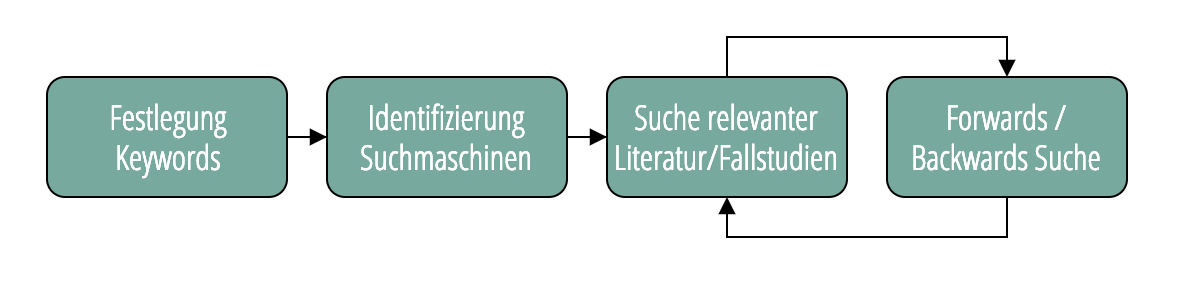
\includegraphics[width=0.8\linewidth]{pics/suchstrategie}}
	\caption[Suchstrategie des SLR]{Suchstrategie des SLR (eigene Darstellung)}
	\label{fig:suchstrategie}
\end{figure}

Wie der Abbildung zu entnehmen wurden zunächst \textit{Keywords} für die  Literatursuche festgelegt. Diese wurden nach einer ersten Probesuche zunehmend angepasst, bis eine zufriedenstellende Ergebnismaske erzielt wurde. Da in der Suche englische  und deutsche Literatur eingeschlossen wurde, wird im folgenden zwischen englischen und deutschen Keywords unterschieden. In \ref{tab:keywordsslr1} werden nachfolgend die \textit{Keyword-Suchketten} aufgeführt, die in sämtlich genutzten Literatursuchmaschinen verwendet wurden. Die Syntax der Suchketten kann dabei  von Suchmaschine zu  Suchmaschine variieren, die Übersicht dient der Allgemeinheit.

\begin{table}[ht]
	\centering
	\caption{Übersicht Keyword-Suchketten SLR 1}
	\begin{tabular}{|p{7cm}|p{7cm}|}
		\hline
		\textbf{Deutsche Keywords}& \textbf{Englische Keywords} \\
		\hline
		digitale+transformation+fallstudie OR digitalisierung+fallstudie   & digital+transformation+case OR digitalization+case \\
		\hline
	\end{tabular}
	\label{tab:keywordsslr1}
\end{table}

Weiter wurden im Vorfeld relevante Literatursuchmaschinen identifiziert. Dabei wurde darauf geachtet, dass überwiegend Suchmaschinen mit Zugang zur technischer sowie wirtschaftlicher Relevant gewählt wurden. Grundsätzlich wurden überwiegend Datenbanken mit vorhandenem Online-Zugang genutzt. \todo{weiter ausführen?} \ref{tab:suchmaschinenslr1} zeigt hierbei  eine Übersicht der genutzten Suchmaschinen mit Angabe der insgesamt gefundenen Literatur.

\begin{table}[ht]
	\centering
	\caption{Übersicht Literatursuchmaschinen SLR 1}
	\begin{tabular}{|p{5cm}|p{7cm}||p{3cm}|}
		\hline
		\textbf{Datenbank/Bibliothek}& \textbf{URL} &  \textbf{Treffer Keywords  (summiert)} \\
		\hline
		IEEE Xplore & \url{https://ieeexplore.ieee.org} & 770 \\
		(Online) - Bibliothek Hochschule Harz & \url{https://opac.lbs-magdeburg.gbv.de/DB=4/LNG=DU} & 6 \\
		(Online) - Bibliothek Technische Universität Berlin  & \url{https://www.ub.tu-berlin.de/literatur-suchen}& 1 \\
		Google Scholar &  \url{https://scholar.google.de}  & 26.800 \\
		Scopus & \url{https://www.scopus.com} & 4.347 \\
		ResearchGate & \url{https://www.researchgate.net} &Keine Angabe vorhanden \footnotemark \\ 
		ACM Digital Library & \url{https://dl.acm.org} & 174.857 \\
		\hline
	\end{tabular}
	\label{tab:suchmaschinenslr1}
\end{table}

\footnotetext{\textit{ResearchGate} bietet keine Funktion zur Angabe der kompletten Treffer-Zahl}

Des Weiteren beinhaltete der vorgenommene Suchprozess eine sogenannte \textit{Forwards - und Backwards-Suche}. Demzufolge wurden mithilfe der bereits gefundenen Fallstudien weitere, zitierte Studien erschlossen (Backwards). Ebenso wurden mithilfe der Suchmaschinen, insoweit die Funktion bereitgestellt wurde, Fallstudien oder Literatur gesucht, die von den gefunden Fallstudien zitiert wurden (Forwards). So konnte eine große Menge von potentiellen Fallstudien  gefunden werden.

Die Angaben zu den Literatur-Treffern in den einzelnen Suchmaschinen zeigt klar, dass eine weitere Filterung vorgenommen werden musste. Dafür wurden ein \textit{Auswahlprozess} definiert, um nur relevante Fallstudien für die folgenden Untersuchungen zu inkludieren. Dieser wird in \ref{fig:auswahlprozess} dargestellt.

\begin{figure}[H]
	\centering
	\fbox{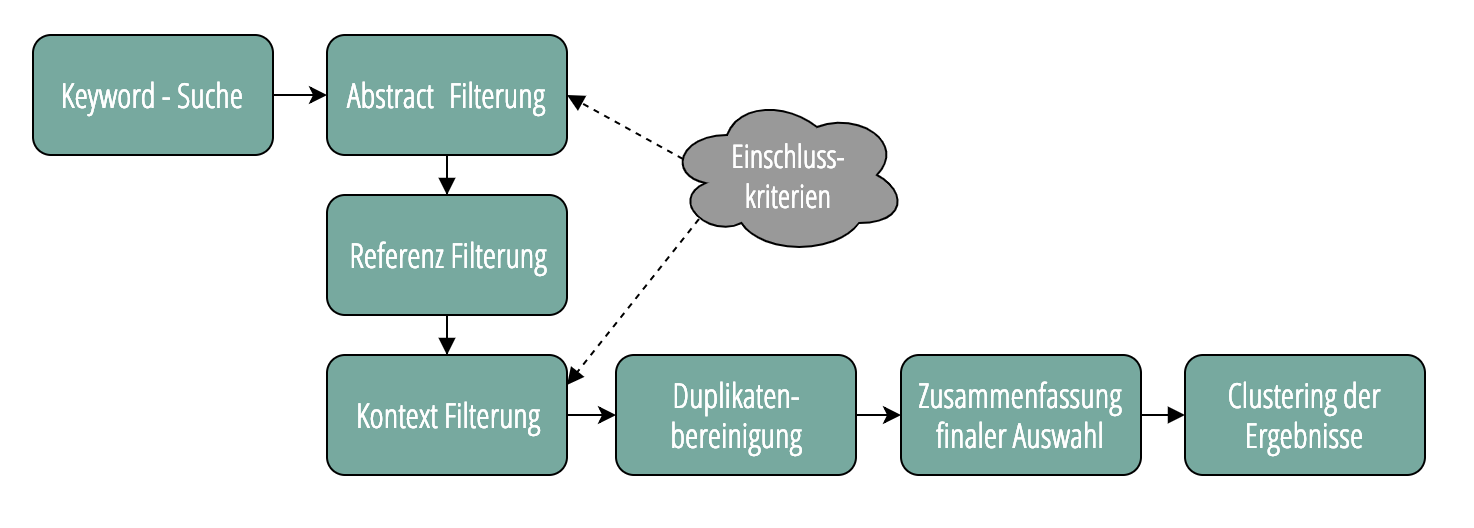
\includegraphics[width=0.8\linewidth]{pics/auswahlprozess}}
	\caption[Auswahlprozess des SLR]{Auswahlprozess des SLR (eigene Darstellung)}
	\label{fig:auswahlprozess}
\end{figure}

Um der großen Menge an Literatur zu begegnen und zu filtern, wurden eine Reihe von Schritten durchgeführt. Wie der \ref{fig:auswahlprozess} zu entnehmen, wurde für die gesamte aus der Keyword-Suche ermittelten Literatur zunächst eine Reihe von \textit{Ein - und Ausschlusskriterien} durchlaufen. Diese bezogen sich zunächst nur auf den Abstract. Sind beispielsweise wesentliche Keywords gar nicht erst wirklich vorhanden, wird die betrachtete Literatur verworfen. Weiterhin wurde überprüft, ob auf eine referenzielle Unverfälschtheit geschlossen werden kann. Dies bedeutet, dass solche Literatur nicht benutzt wird, die augenscheinlich nur eine Kopie einer bereits gefundenen ist; und zwar in dem Zusammenhang, als das sie gegenseitig im Literaturverzeichnis vorkommen. An dieser Stelle sei gesagt, dass dieser Fall sehr vermindert aufgetreten ist. 

Des Weiteren wurden die Ein - und Ausschlusskriterien auf den eigentlichen Inhalt jeder Literatur angewendet. Im Anschluss wurden eine weitere Duplikatenbereinigung durchgeführt. Als Ergebnis dieser Filterungsschritte konnte eine viel kleinere Stückzahl an Fallstudien gewonnen, diese zusammengefasst und geclustert werden.

Im folgenden soll auf die genutzten Ein - und Ausschlusskriterien eingegangen werden. \ref{tab:criteriaslr1} zeigt eine Übersicht der genutzten Kriterien. Grundsätzlich wurde keine Einschränkung in Bezug auf die Nationalität des beschriebenen Unternehmens gemacht. Ebenso gab es keine Beschränkung auf die Branche. Im Bezug auf die \textit{Empirik} wurden nur Fallstudien oder Studien zugelassen. Ebenso mussten alle Objekte eine klare Methodik vorweisen. Demzufolge musste jeweils klar erkenntlich sein, was untersucht wurde und mit welchen wissenschaftlichen Mitteln. Inhaltlich mussten sich die (Fall-)Studien auf die  Implementation einer Digitalen Transformation in einem Großunternehmen drehen. Studien zu KMU wurden  nur dann einbezogen, wenn ein klarer Bezug zu einem größeren Kontext gegeben ist, beispielsweise durch Ausführungen für eine mögliche Skalierung der gefundenen Ergebnisse. Außerdem wurden nur solche Fallstudien inkludiert, die  gesamtorganisationale Schwerpunkt setzen. Dies bedeutet, dass nicht nur auf die Implementation einzelner Technologien, wie beispielsweise \textit{Big Data} eingegangen werden sollte. Ein Bezug auf  das gesamte Unternehmen muss klar erkenntlich sein. Hinsichtlich der gewählten Sprache musste die Literatur auf deutsch oder englisch sein. Das Veröffentlichungsdatum durfte nicht vor dem Jahr 2014 liegen, um eine gewisse Aktualität zu gewährleisten.

\begin{table}[ht]
	\centering
	\caption{Ein - und Ausschlusskriterien SLR 1}
	\begin{tabular}{|p{4cm}|p{8cm}|}
		\hline
		\textbf{Kriterium}& \textbf{Erklärung}  \\
		\hline
		Empirik & Literatur muss eine Fallstudie oder Studie sein \\
		Wissenschaftlichkeit & Methodik der  Fallstudie oder Studie muss klar erkennbar sein \\
		Kontext & inhaltlich Digitale Transformation in Großunternehmen; Mittelständische nur dann, wenn relevant für größeren Kontext \\
		Allgemeinheit & keine Spezifität von einzelnen technischen Implementationen, Gesamtorganisationaler Kontext muss vorhanden sein \\
		Sprache & deutsch oder englisch \\
		Aktualität & ab 2014 - heute  \\
		\hline
	\end{tabular}
	\label{tab:criteriaslr1}
\end{table}

Durch die genutzten Ein - und Ausschlusskriterien konnte die große Menge an Literatur auf eine kleine Gruppe relevanter Fallstudien und Studien im Themenfeld der Digitalen Transformation von Großunternehmen heruntergebrochen werden. Insgesamt konnten \textit{23} Literaturobjekte gefunden werden. Diese beinhalten zusammen rund \textit{200} Fallstudien zu Großunternehmen in verschiedenen Bereichen.

\section{Literaturübersicht}

% - Fallstudien
% - tabellarische Darstellung (https://docs.google.com/document/d/1caHZ-pLGa\_L-TfO4nOh2zZLdAa5nazKaoUZDeDmN90M/edit)
% - Inhaltsangabe jeder Arbeit (Zusammenfassung)

Nachfolgend soll eine kleine Übersicht der gefundenen und gefilterten Literatur gegeben werden, die für die weiteren Untersuchungen verwendet wurden. Eine große Übersicht der  Bücher, wissenschaftlichen Artikeln u.a. findet sich in \ref{tab:overviewliterature1} und \ref{tab:overviewliterature1-2} im Anhang. Diese beinhaltet neben Autor und Titel jeder Publikation eine kurze Übersicht zum Untersuchungsgegenstand.

Wie im vorangestellten Abschnitt bereits aufgeführt, wurden insgesamt 23 (Fall-)Studien ausgewertet. Jede eingeschlossene Publikation muss zumindest in ausgewählten Abschnitten Fallstudien zum dargestellten Thema beinhalten. Nachfolgend soll für jede eine kurze inhaltliche Beschreibung gegeben werden.

\citeA{muchna_aspekte_2018} thematisieren in ihrer Arbeit grundsätzliche Aspekte des Zusammenwirkens von Innovations- und Change Management. Gesondert im 7. Kapitel wird eine Fallstudie der Digitalen Transformation des Deutschen Banksektors  beschrieben. Es wird auf aktuelle Herausforderungen Chancen und Best Practices im Bezug auf die Digitalisierung für diese Branche eingegangen.

Ein sehr übersichtlichen Beitrag zu Fallstudien innerhalb der Digitalen Transformation von Großunternehmen stellen \citeA{gassmann_digitale_2016} in ihrem Buch bereit. Besonders im zweiten Teil werden gleich 11  Fallstudien zu dieser Thematik dargestellt. Es wird systematisch auf Erfolgsfaktoren und Handlungsanweisungen für  eine erfolgreiche Digitale Transformation hingewiesen, jedoch auch auf Hürden und Probleme eingegangen.

\todo{u.a. ab 3 Autoren!}
Eine weiteren Fall beschreiben \citeA{chanias_digital_2018} in ihrer Arbeit. Es geht zwar hierbei um die Digitale Transformation eines mittelständischen, europäischen Anbieter im Finanzwesen, jedoch werden die Ergebnisse weiterführend in Form von allgemeinen Problematiken und Handlungsempfehlungen auf einen großen Kontext geschlossen. Damit gelten die Ein - und Ausschlusskriterien (vgl. \ref{problemfields:methods}) als erfüllt.

Eine ganze Reihe von Fallstudien präsentieren \citeA{urbach_digitalization_2018} in ihrer Publikation. Es werden gleich 21 Fälle der Digitalen Transformation von Großunternehmen präsentiert. Hierbei wurde sehr systematisch vorgegangen und  wiederkehrend auf Probleme, Lessons Learned und Best Practices eingegangen.

Insgesamt 9 internationale Fälle bietet das Werk von \citeA{gartner_fallstudien_2018}. Interessant ist hierbei  zudem, dass in allen Fällen direkt auf den Einfluss des Mitarbeiters als Menschen eingegangen wurde.

\citeA{oswald_digitale_2018} beschreiben im vierten Teil ihres Buches 4 Fallstudien aus dem deutschsprachigen Raum. Es wird außerdem angegeben, dass insgesamt Erfahrungen aus 59 Unternehmen und die Erhebung einer Studie von 650 Organisationen in der Automobilbranche für die Erstellung der Fallstudien eingeflossen sind.

Eine große Studie führten außerdem \citeA{hoberg_skills_2017} durch und veröffentliche die Ergebnisse in seiner Arbeit. Insgesamt wurden 116 Vertreter von Unternehmen aus 18 Ländern befragt. Die Ergebnisse zeigen klare  Trends in der Implementation der Digitalen Transformation, aber weist auch vermehrt auf Probleme bin.

Eine weitere Studie führten \citeA{solis_2017_2017} durch. Insgesamt wurden 528 Offizielle von Unternehmen aus 5 großen Industriestaaten befragt. Die Ergebnisse zeigen gegenwärtige Entwicklungen innerhalb der Digitalen Transformation der befragten Unternehmen.

\citeA{kremins_2018_2018} führte eine Studie innerhalb der internationalen Reisebranche durch. Insgesamt wurden rund 200 Unternehmen befragt. Als Ergebnisse werden Probleme und Handlungsempfehlungen dargestellt.

Im Bezug auf die Handelsbranche stellten \citeA{heinemann_digitale_2016} insgesamt 15 Fallstudien von internationalen Großunternehmen in dieser Branche zusammen. Es wird systematisch auf Probleme und Handlungsempfehlungen eingegangen.

\citeA{nowik_promoting_2018} fasst in seiner Arbeit die Ergebnisse einer Studie mit 8 schwedischen Großunternehmen aus der Finanzbranche zusammen. Es wird schwerpunktmäßig auf Probleme und Gründe eingegangen, warum bestimmte Firmen im Transformationprozess zunehmend hinter ihrer Konkurrenz liegen.

Im Transformationswerk des Jahres 2016 stellen \citeA{buhse_transformationswerk_2016} eine Studie mit 1060 Vertretern von deutschen Groß - und mittelständischen Unternehmen vor. Es wird  verstärkt auf Problematiken im Transformationsprozess, aber auch auf Treiber und Handlungsweisungen eingegangen.

Eine große Fallstudie präsentiert \citeA{wautelet_impact_2017} in seiner Arbeit. Es wird zunächst auf die Notwendigkeit der Digitalen Transformation des dargestellten Unternehmens, dann auch auf Probleme und Lessons Learned eingegangen.

Die Ergebnisse von insgesamt 82 Fallstudien fasst die Arbeit von \citeA{weber_digital_2015} zusammen. Alle betrachteten Unternehmen kommen aus dem Fertigungs-,  Dienstleistungs-,  sowie dem Informations - und Kommunikationstechnologie-Sektor (IKT). Es werden wichtige Handlungsfelder und Grundlagen für den Erfolg der Digitalen Transformation dargestellt.

Insgesamt 3 Medienkonzerne aus dem deutschsprachigen Raum stellt \citeA{hess_options_2016} in seiner Publikation dar. Es wird auf Probleme  und wichtige Treiber der Transformation in diesen Unternehmen eingegangen.

Eine weitere Studie zum Status der Digitalen Transformation in Deutschland stellt \citeA{depiereux_studie_2018} vor. Insgesamt wurden 2000 Unternehmen befragt. Es wird auf wichtige gegenwärtige Probleme eingegangen.

\citeA{buxmann_digitalisieren_2016} beschreiben in ihrer Arbeit die Ergebnisse einer Studie mit 103 Großunternehmen aus der deutschen Maschinen- und Anlagenbau-, Automotive- sowie Logistik/Transport-Branche. Es wird darauf hingewiesen woran es zunehmend im Transformationsprozess mangelt und an welchen Punkten für einen erfolgreichen Wandel gearbeitet werden muss.

Insgesamt 5 Fallstudien aus dem deutschsprachigen Raum zeigen \citeA{berghaus_2016} in ihrer Veröffentlichung. Es werden systematisch Erfahrungsberichte aufgezeigt. Interessant ist hierbei besonders die Erkenntnis, dass oftmals ein klares  Ziel beim Transformationsprozess fehlt.

Eine Übersicht im Bezug zur Digitalen Transformation aller 30 DAX-Unternehmen stellen \citeA{kawohl_digitale_2016} vor. Es wird auf den aktuellen Status der Unternehmen im Transformationsprozess eingegangen, sowie  auf  Probleme und Handlungsweisungen.

\citeA{beule_digital_2019} thematisieren in ihrer  Arbeit die Erkenntnisse von 6 Fallstudien von internationalen Unternehmen in der Radiobranche. Das Ziel war hierbei, Problemfelder zu identifizieren und Lösungsvorschläge zu präsentieren.

Im dritten Teil ihrer Arbeit stellen \citeA{oswald_shaping_2017} insgesamt 3  Fallstudien zu Großunternehmen vor. Es wird  auf die Bedeutung der Transformation, sowie im einzelnen auf Probleme und Handlungsempfehlungen eingegangen.

Eine weitere Fallstudie präsentieren \citeA{savastano_how_2018} in ihrer Arbeit. Das beschriebene Unternehmen befindet sich in der Ernährungsbranche. Es wird verstärkt auf Probleme und wichtige Lessons Learned eingegangen.

Als letzte Publikation wurde die Arbeit von \citeA{macgillavry_digital_2014} eingeschlossen. Sie beschreiben eine Fallstudie eines großen, internationalen Unternehmens aus der Logistikbranche. Es werden Herausforderungen, aber auch wichtige Handlungsempfehlungen gegeben.

Insgesamt bieten alle gefundenen und eingeschlossenen Publikationen eine sehr große Vielfalt an Erkenntnissen, die im folgenden in zwei Schritten zusammengefasst und geclustert werden sollen.

\section{Veränderungsprozessmuster innerhalb der Digitalen Transformation}
\label{problemfields:changepatterns}

Nachdem im vorangestellten Abschnitt die  gewählte Literatur inhaltlich kurz  beschrieben wurde, sollen die Ergebnisse aller (Fall-) Studien nun zusammengefasst werden. Zunächst sollen sogenannte \textit{Veränderungsprozessmuster} erschlossen werden. Wie in \ref{introduction} bereits angeklungen, beziehen sich solche Muster auf wiederkehrende Bereiche, die innerhalb der Digitalen Transformation verändert bzw. digitalisiert werden. Alle 23 Publikationen wurden genau studiert  und die genannten Felder der Veränderung extrahiert.

Eine vollständige Auswertung darüber, welche Veränderungsprozessmuster in welcher Literatur genannt wurden, findet sich in \ref{tab:clusteringchangeprocess} im Anhang anhand einer Kreuzmatrix. Eine vereinfachte Übersicht findet sich nachfolgend in \ref{tab:clusteringvpshort}. Die Übersicht zeigt den Versuch eines Clusterings, d.h. einer Zusammenfassung der Nennungen gleichartiger  Veränderungsprozessmuster. 

\begin{table}[ht]
	\centering
	\caption{Auswertung Clustering Veränderungsprozessmuster (kurz)}
	\begin{tabular}{|c|c|}
		\hline
		\textbf{Veränderungsprozessmuster}& \textbf{Anzahl Nennungen} \\
		\hline
		Einführung einer Multi-Kanal-Strategie   & 6  \\
		Wechsel vom Offline- zum Online-Vertrieb & 5  \\
		Erschaffung neuer digitaler Produkte     & 12 \\
		Tendenz zur Kundenorientierung           & 16 \\
		Digitalisierung des Geschäftsmodell      & 11 \\
		Digitaler Wissensaufbau im Unternehmen   & 12 \\
		Datengestützte Verbesserungsprozesse     & 5  \\
		Erzeugung eines digitalen Ökosystems     & 7  \\
		Digitalisierung von internen Prozessen   & 7  \\
		Einbindung innovativer Technologien      & 6  \\
		Aufbau technisches Sicherheitskonzept    & 4  \\
		Digitale Neuausrichtung der Organisation & 13 \\
		Innovationsförderung                     & 7  \\
		Kooperation mit externen Treibern        & 5 \\
		\hline
	\end{tabular}
	\label{tab:clusteringvpshort}
\end{table}

Insgesamt konnten \textit{14} verschiedene Felder der Veränderung durch die Digitale Transformation anhand des SLR bestimmt werden. Diese Gruppe bildet eine Auswahl von oft genannten Varianten. Mehrere, nur einmalig genannte  Veränderungen wurden in der Auswertung vernachlässigt.

Jedes einzelne beschreibt eine Maßnahme bzw. eine Facette des vom Transformationsprozess beeinflussten Unternehmens.  Ebenfalls zeigt die \ref{tab:clusteringvpshort} die Anzahl, in welchen Literaturquellen das jeweilige Muster direkt genannt wurde. Oft ergaben sich diese aus den Beschreibungen über die genauen Vorhaben der Transformation. 
In vielen Fällen lässt sich der Begriff der \textit{Digitalisierung} erkennen. Dies ist durchaus nachvollziehbar, da dieser Schwerpunkt stark mit der Digitalen Transformation einhergeht (vgl. \ref{background:dt}). Nachfolgend soll auf jedes Muster kurz eingegangen werden, um ein besseres Verständnis zu schaffen.

\todo{Wenn noch Platz, gerne für jeden Punkt noch Zitate aufführen. }
% https://docs.google.com/document/d/1caHZ-pLGa_L-TfO4nOh2zZLdAa5nazKaoUZDeDmN90M/edit#

Als erstes kann die \textit{Einführung einer Multi-Kanal-Strategie} als eine Aktion der Digitalen Transformation genannt werden. Hierbei geht es grundlegend darum, neue  Wege des Vertriebs der eigenen Produkte zu erschließen \cite[S. 242]{muchna_aspekte_2018}. Darüber erhoffe man sich, neue Schnittstellen zum Kunden zu gewinnen; gerade durch das Aufkommen des Online-Vertriebs und Sozialen Medien \cite[S. 21]{solis_2017_2017}.

Eng damit verbunden erscheint das Muster des \textit{Wechsels vom Offline - zum Online-Vertrieb}. Nicht nur, dass Unternehmen dazu neigen, neue Online-Angebote zu bieten, alte Vertriebskanäle werden teilweise komplett aufgelöst. \citeA{oswald_digitale_2018} führen in ihrer Fallstudie zur deutschen Finanzbranche beispielsweise auf, dass klassische Bankprodukte vermehrt  mit digitalen Varianten ersetzt werden (S. 146).

Dazu gehört selbstverständlich auch die \textit{Erschaffung neuer digitaler Produkte}. Kunden sind es mit dem Aufkommen neuer technischer Möglichkeiten gewohnt, digitale Produkte zu nutzen. Demnach ist ein Umdenken in diese Art der Produktentwicklung unumgänglich, beispielsweise durch das Angebot digitaler Medien \cite[S. 303]{heinemann_digitale_2016}. 

Im Bezug auf das Angebot von digitalen Produkten geht auch die steigende \textit{Tendenz zur Kundenorientierung} einher. Es wird zunehmend wichtiger, den Kunden aktiv in die Produktentwicklung zu integrieren \cite[S. 17]{depiereux_studie_2018}. Nur zu erziele man ein wirkliches Kundenerlebnis und neue Anreize, Produkte verkaufen zu können, wovon betriebswirtschaftlich letztendlich der Unternehmenserfolg abhängt.

Eine andere Variante von digitalen Produkten kann auch die allgemeine \textit{Digitalisierung des aktuellen Geschäftsmodells} sein. Bietet das Unternehmen beispielsweise Dienstleistungen an, wird es zunehmend zum Trend, diese auch über eine digitale Form anzubieten. Zum Beispiel beschreiben \citeA{oswald_digitale_2018} in einer ihrer Fallstudien, wie ein Unternehmen den Verkauf von Druckluft umgestellt hat (S. 100). Nach dem Prinzip von \textit{Druckluft as a Service} wird dieser nicht mehr zu einem Festpreis verkauft, sondern der Preis kann durch neuartige Auswertungsmethoden dynamisch angepasst werden.

Zu jedem Veränderungsprozess gehört das nötige  Know-How. Demzufolge erscheint es nicht ungewöhnlich, dass der \textit{Digitale Wissensaufbau im Unternehmen} ebenfalls als oft genanntes Muster. Die Maßnahmen in diesen Bereich fielen sehr unterschiedlich aus. Beispielsweise wurden Workshops zur Schulung neuer digitaler Fähigkeiten für alle oder ein Teil der Mitarbeiter durchgeführt \cite[S. 177]{gassmann_digitale_2016}. Teilweise wurden sogar komplett neue Teams zusammengestellt, um die Digitale Transformation gezielt zu steuern \cite[S. 139]{urbach_digitalization_2018}. Es geht grundsätzlich darum, dem Unternehmen das nötige Rüstzeug für die Transformation zu geben, sei es durch den Einkauf von Know-How oder durch interne Schulungen.

Oft genannt wurden auch die Maßnahme der kontinuierlichen \textit{Verbesserungsprozesse} (KVP). Diese sind durchaus keine neue Erfindung, im Bezug auf die geschilderten Transformationsprozesse kristallisiert sich  aber die  Besonderheit heraus, dass diese zunehmend \textit{datengestützt} ist. Durch neue technologische Möglichkeiten wie beispielsweise \textit{Big Data} hat man somit die Möglichkeit, ganz neue Daten und Metriken zum Veränderungsprozess oder allgemein zum Unternehmen zu erheben und regelmäßige Feedback-Schleifen zu erstellen \cite[S. 8]{beule_digital_2019}.

Interne Veränderungen wurden ebenfalls mehrfach genannt. Dabei fiel oft die Begrifflichkeit der \textit{Erzeugung eines digitalen Ökosystems}. Dies bedeutet im Wesentlichen, dass interne Prozesse mit dem eigenen Leistungsangebot an Produkten stark verdrahtet werden \cite[S. 127]{heinemann_digitale_2016}. Dieses Modell kommt somit einer großangelegten Digitalen Transformation am nächsten, in dem digitale Produkte geschaffen werden, Netzwerke gebildet und Verbindungen zwischen internem und externem Schaffen erzeugt werden. Man kann das digitale Ökosystem somit als einer Art Verknüpfung aller hier genannten Muster verstehen.

Neben der Digitalisierung  von Dienstleistungen, Produkten und generell das eigene Geschäftsmodell, gehört auch die \textit{Digitalisierung von internen Prozesses} zum Rahmen der Digitalen Transformation. Beispielsweise durch das Aufkommen von \textit{Robotic Process Automation} (RPA) oder \textit{Predictive Maintenance} erhält man komplett neue Möglichkeiten, die eigene Wertschöpfungskette, aber auch generelle unternehmensweite Geschäftsprozesse  stetig zu optimieren \cite[S. 16f.]{urbach_digitalization_2018}.

Zur generellen Definition der Digitalen Transformation gehört natürlich auch die \textit{Einbindung innovativer Technologien}. Beispielsweise wird \textit{Big Data} genutzt, um in verschiedensten Abteilungen neue Kenntnisse zu gewinnen und Innovationen voranzutreiben \cite[S. 22]{gartner_fallstudien_2018}. Oft werden dieser aber auch genutzt, um die eigene IT-Infrastruktur auszubauen \cite[S. 8]{chanias_digital_2018}. Unternehmen sollen demnach stetig versuchen, gegenwärtige Trends aufzunehmen und in ihr Geschäftsmodell zu integrieren \cite[S. S. 89]{gartner_fallstudien_2018}.

Das Thema Sicherheit hat im Bereich der Digitalisierung ebenfalls eine hohe Wichtigkeit. Deswegen erscheint es nicht überraschend, dass der \textit{Aufbau eines technischen Sicherheitskonzepts} ebenfalls als ein Veränderungspunkt mehrfach genannt wurde. Wichtig erscheint vielen Unternehmen, Informationen sicher und vertrauenswürdig zu behandeln \cite[S. 8]{weber_digital_2015}. Der Bereich des Datenschutzes von Kunden-, aber auch von Mitarbeiterdaten ist ein zunehmend wichtiges Thema.

Folgender Punkt ist bereits durch die Schaffung eines digitalen Ökosystems angeklungen. Trotzdem ist eine \textit{digitale Neuausrichtung der Organisation} weiterhin erwähnenswert. In einer Reihe von Fallstudien wurden gesonderte Umstrukturierungen der IT-Abteilung genannt \cite[S. 393]{urbach_digitalization_2018}.  Teilweise wurden auch eigene Divisionen für den Transformationsprozess geschaffen \cite[S. 8]{beule_digital_2019}, aber auch komplette Organisationen umgestellt \cite[S. 4]{kawohl_digitale_2016}. Letzteres steht auch im Zusammenhang mit denen im \ref{background:agileorganisation} geschilderten Beispielen. Es ginge grundsätzlich darum, die Organisation bereit für anstehende Veränderungen zu machen \cite[S. 31]{berghaus_2016}

Um wettbewerbsfähig zu bleiben, setzen immer mehr Unternehmen auf eine stetige \textit{Innovationsförderung}. Durch Kooperationen, gezieltes Management oder die Einrichtung von Innovationszentren soll das Schaffen neuer Ideen zunehmend gefördert werden \cite[S. 33]{buxmann_digitalisieren_2016}. Man erhoffe sich so eine Entstehung einer Innovationskultur im Unternehmen.

Als letzter, mehrfach genannter Veränderungspunkt soll die \textit{Kooperation mit externen Treibern} genannt werden. Hierbei geht  es nicht nur um die Bestellung von externen Beratern beim Veränderungsprozess, sondern auch die direkte Kooperation mit \textit{Start-Ups} oder einer eigenen \textit{Open Source Community} \cite[S. 139]{urbach_digitalization_2018}. Man erhoffe sich hierdurch stärkende Einflüsse von außen, ohne große Anstrengungen ins eigene Wissensmanagement stecken zu müssen. Dieses Muster kann teilweise als Gegenentwurf zum digitalen Wissensaufbau gesehen werden, wobei Symbiosen auch denkbar sind \cite[S. 154]{urbach_digitalization_2018}.

Die dargestellten Veränderungsmuster lassen erahnen, dass eine Vielzahl von Veränderungen innerhalb des Transformationsprozesses geben kann. Interessant ist hierbei, dass die \textit{Tendenz zur Kundenorientierung} am meisten genannt wurde. Dies lässt erahnen, dass viele Unternehmen in diesem Thema das größte Potenzial sehen, um neue Geschäftsbereiche und Produktangebote zu erschließen.

Die erarbeiten Muster der Veränderung werden in der Erstellung von Best Practices (vgl. \ref{agilepractices}) teilweise nochmal aufgegriffen. Nachfolgend sollen nun bestimmte Problemfelder in den getroffenen  Veränderungen erarbeitet werden.

\section{Identifikation von Problemfeldern}


Im vorangegangen Abschnitten wurden zunächst Ansatzpunkte für mögliche Veränderungen in der Digitalen Transformation genannt. Als nächster Schritt des vorliegenden SLR wurden innerhalb der Publikationen mögliche Problemfelder im Transformationsprozess gesucht. Ähnlich wie im ersten Teil wurde versucht, gleichartige Problemfelder zu clustern. Eine vollständige Auswertung in Form einer Kreuzmatrix findet sich in \ref{tab:clusteringproblemfields} im Anhang. Nachfolgend soll \ref{tab:clusteringpfshort} eine vereinfachte Übersicht über die gefundenen  Problemfelder geben. Wieder wurden einfach genannte Untersuchungsobjekte vernachlässigt. Als nächster Schritt  der Ergebnisaufbereitung sollen alle Problemfelder nun kurz erläutert werden.

\begin{table}[ht]
	\centering
	\caption{Auswertung Clustering Problemfelder (kurz)}
	\begin{tabular}{|c|c|}
		\hline
		\textbf{Problemfeld}& \textbf{Anzahl Nennungen} \\
		\hline
		Unternehmensweite Kommunikationsprobleme        & 5  \\
		Festhalten an verfestigten Strukturen           & 7  \\
		Zeit - und Marktdruck                           & 5  \\
		Unterschätzung der Komplexität                  & 4  \\
		Fehlende Kontinuierliche Verbesserungsprozesse  & 7  \\
		Störung durch oberes Management (Top-Down)      & 7  \\
		Konflikte zwischen IT und Business              & 4  \\
		Fehlende frühe Einbeziehung aller Mitarbeiter   & 3  \\
		Sicherheitsprobleme                             & 2  \\
		Fehlende Kundenorientierung                     & 13 \\
		Fehlendes technisches Know-How                  & 10 \\
		Fehlende monetäre Ressourcen                    & 2  \\
		Rechtliche Bestimmungen und Datenschutz         & 5  \\
		Fehlende Transparenz (intern und extern)        & 4  \\
		Fehlende Partnerschaften                        & 6  \\
		Fehlende Innovationskultur                      & 6  \\
		Langsame Entscheidungsprozesse                  & 3  \\
		Unternehmenskulturelle Probleme                 & 8  \\
		Fehlendes Vertrauen, Akzeptanz und Bereitschaft & 9  \\
		Unklare Verantwortlichkeiten                    & 5  \\
		Fehlende digitale Strategie                     & 6 \\
		\hline
	\end{tabular}
	\label{tab:clusteringpfshort}
\end{table}

\todo{Wenn noch Platz, gerne für jeden Punkt noch Zitate aufführen. }
% https://docs.google.com/document/d/1caHZ-pLGa_L-TfO4nOh2zZLdAa5nazKaoUZDeDmN90M/edit#

Im ersten Punkt der \textit{unternehmensweiten Kommunikationsprobleme} spiegeln sich schon klassische Probleme im Change Management wieder. Oft mangelte es schon am Vorhanden sein von funktionierenden Kommunikationskanälen in allen Bereichen des Unternehmens \cite[S. 234]{muchna_aspekte_2018}. 

Gerade im Hinblick auf die drastischen Veränderungen in der Digitalen Transformation verhindert das \textit{Festhalten an verfestigten Strukturen} einen erfolgreichen Ablauf. Es zeigte sich oft, dass funktionierende Geschäftsmodelle nicht aufgebrochen werden wollen \cite[S. 194]{gassmann_digitale_2016}. Dies verhindert das Aufkommen von Bereitschaft für Veränderungen in der Führungsetage und somit überhaupt die Chance auf einen gut ablaufenden Transformationsprozess.

In vorher liegenden Abschnitten ist bereits angeklungen, dass die Digitale Transformation ein langwieriger Prozess ist. Gerade in hartumkämpften Branchen ist der \textit{Zeit - und Marktdruck} ein großes Problem für das Change Management. Beispielsweise fordert ein digitalisiertes Produktsortiment eine längere Zeitspanne bis zum Markteintritt \cite[S. 183]{urbach_digitalization_2018}.

Viele Unternehmen unterschätzten schlichtweg die \textit{Komplexität} der Digitalen Transformation. Einerseits mangelte  es an der Berücksichtigung der gesamten Organisation in die Veränderungen; teilweise wurde zunächst nur die IT-Abteilung angegangen; auch das Maß an sozialen Veränderungen wurde komplett unterschätzt \cite[S. 4]{hoberg_skills_2017}.

Es fehlte zudem an \textit{kontinuierlichen Verbesserungsprozessen}. Innerhalb eines Change-Management-Prozesses bedarf es an regelmäßigen Feedback-Schleifen, um die getätigten Veränderungen dauerhaft zu evaluieren \cite[S. 13]{kaune_change_2016}. Eine funktionierende Digitale Transformation sollte kontinuierlich überprüft werden, aus Fehlern sollte  durchgängig gelernt werden \cite[S. 15]{chanias_digital_2018}.

Vorangetriebene Veränderungsinitiativen scheiterten oft durch \textit{Störungen des oberen Managements}, was oft am Festhalten an alte Strukturen und die dadurch fehlende Bereitschaft für Veränderungen lag. Die firmeneigene Politik oder schlichtweg Egos verhinderten ein Gelingen der Initiativen \cite[S. 4]{solis_2017_2017}.

Gerade bei einem so einem interdisziplinären Thema wie die Digitale Transformation kann es zu \textit{Konflikten zwischen IT und Business} kommen. Es kam zu unterschiedlichen Vorstellung, wie ein neues Geschäftsmodell aufzubauen ist, gerade  im Hinblick auf technischer Machbarkeit und Wirtschaftlichkeit \cite[S. 117]{oswald_digitale_2018}.

Der Bereits angeklungene Widerstand für geplante Veränderungen kann auch durch eine \textit{fehlende frühe Einbeziehung aller Mitarbeiter} entstehen. Schafft man es nicht, die Belegschaft  für anstehende technische Änderungen zu motivieren, wird man diese nicht vorantreiben können \cite[S. 40]{kawohl_digitale_2016}. Interessant ist dieser Punkt gerade deshalb, weil er dafür spricht, dass oft ein Top-Down-Ansatz für den Veränderungsprozess gewählt wurde.

Auch können \textit{Sicherheitsprobleme} gegen eine erfolgreiche Implementation neuer Technologien gewirkt haben. Beispielsweise berichten \citeA{urbach_digitalization_2018} in einer ihrer Fallstudien von derartigen Problemen. Solche können natürlich dazu führen, dass das Vertrauen in neuartigen Technologien sinkt, was Veränderungen bremsen kann.

Im Bereich der Veränderungsprozessmuster (vgl. \ref{problemfields:changepatterns}) fiel die \textit{Kundenorientierung} bereits durch eine hohe Zahl an Nennungen auf. Deswegen erscheint es nicht verwunderlich, dass hier auch ein großes Problem liegen kann. Wird der Fokus hier nicht gelegt, bzw. wird dieser Punkt komplett vernachlässigt, werden Nachteile sichtbar. Können beispielsweise neue Produkte nicht ausreichend personalisiert werden, verliert man den direkten Kontakt zum Kunden \cite[S. 20]{kremins_2018_2018}.

Oft scheitert es bei der Umsetzung schon am nötigen Wissen. So wurde auch ein \textit{fehlendes technisches Kno-How} mehrfach als Problem in der Digitalen Transformation genannt. Entweder wurde intern nicht genug für den technischen Wissensaufbau getan, oder es fehlte am Recruiting fachspezifischer Mitarbeiter \cite[S. 37]{kawohl_digitale_2016}.

Neben der Komponente Zeit fehlte es  manchen Unternehmen auch an \textit{monetären Ressourcen}. Beispielsweise berichten \citeA{urbach_digitalization_2018} in einer ihrer Fallstudien ober solch ein Fehlen. Interessant ist hierbei, dass dieses Problemfeld insgesamt nicht sehr oft genannt wurde. Dies lässt darauf schließen, dass grundsätzlich ein hohes Budget für die Veränderungen bereitgestellt wird.

Gerade im deutschsprachigen Raum wurden \textit{rechtliche Bestimmungen und Datenschutz} als große Hindernisse genannt. Sicherheitsanforderungen beim Einsatz neuer Technologien blockieren die erfolgreiche Integration \cite[S. 7]{depiereux_studie_2018}. Somit wird nicht genügend Raum für einen weitgreifenden Einsatz gegeben, was zur Schwächung im internationalen Marktvergleich führt.

Oft wurden Veränderungen nicht \textit{transparent} gemacht. Weder gab es intern eine genügende Berichterstattung über anstehende Veränderungsprozesse, noch wurde extern damit richtig umgegangen. Ein Beispiel zeigt sich vor allem in der Fallstudie von \citeA{hofert_agile_2018} über die deutsche Finanzbranche, in der eine mangelnde Offenheit nach außen kritisiert wurde.

Im Bezug auf ein fehlendes technisches Know-How können auch \textit{fehlende Partnerschaften} Rechnung tragen. Kann nicht für ein ausreichenden Wissensaufbau im Unternehmen gesorgt werden, kann zumindest durch Partnerschaften nach außen eine solche Lücke geschlossen werden. Wird hier aber auch kein Anstoß geben, fehlt es grundsätzlich an den nötigen Fähigkeiten für die geplanten Veränderungen \cite[S. 9]{nowik_promoting_2018}.

Im Bezug auf das Management ist es stets wichtig, flexibles zu bleiben und immer neue Möglichkeiten für Marktvorteile zu sichern. Ein Ansatzpunkt dafür kann das Aufleben einer \textit{Innovationskultur} sein. Das Fehlen dieser führt dazu, dass durchgeführte Veränderungen ohne dauerhaften Effekt bleiben \cite[S. 25]{weber_digital_2015}. Dies kann im Extremfall sogar zur Marktverdrängung durch innovativere Kontrahenten führen.

Das bereits genannte Festhalten an alten Strukturen führt unter Umständen zu \textit{langsamen Entscheidungsprozesses}. Will man beispielsweise kleine Veränderungen in bestimmten Bereichen vorantreiben, können solche Strukturen stark behindern. Lange Entscheidungswege tragen Sorge dafür, dass bestimmte Veränderungen niemals richtig durchgeführt werden \cite[S. 12]{depiereux_studie_2018}. Das Unternehmen wirkt dadurch grundsätzlich zu festgefahren und unflexibel (ebenda).

Will man gesamtorganisationelle Veränderungen anstreben, brauch es den Aufbau einer neuen \textit{Unternehmenskultur}. Das Finden einer solchen ist oft selbst mit vielen Problemen behaftet. Oft müssen erst die richtigen Hebel in Gang gesetzt werden, damit die Organisation; und die Mitarbeiter selbst; bereit für eine neue Kultur sind \cite[S. 30]{kremins_2018_2018}.

Stark im Zusammenhang mit bereits genannten Problemen steht auch das des \textit{fehlenden Vertrauens, Akzeptanz und Bereitschaft}. Oft zeigt sich Widerstand gegenüber den geplanten Veränderungen. Begegnet man diesem nicht, wird es schwierig, Planungen umzusetzen.  ''Um potenziellen oder tatsächlichen Widerstand zu bearbeiten`` so \citeA{kaune_change_2016},  ''ist somit u. a. eine gezielte Informations- und Kommunikationsstrategie sinnvoll`` (S. 18).

Oft ist innerhalb der Digitalen Transformation nicht klar, wer der eigentliche  Treiber der Veränderung sein soll. Solch \textit{unklare Verantwortlichkeiten} führten oft dazu, dass Prozesse gebremst wurden. Es kam teilweise sogar zu falschen Schuldzuweisungen, was somit ebenfalls zu großen Problem führte \cite[S. 24]{buhse_transformationswerk_2016}.

Als letzter Punkt soll die \textit{fehlende digitale Strategie} genannt werden. Dieses Problemfeld wirkt im ersten Moment ein wenig suspekt, sollte man sich im Unternehmen doch im Klaren sein, wie die Digitale Transformation angegangen werden, und was genau verändert werden soll. Tatsächlich wurde oftmals genannt, dass nicht mal dies im Vornherein klar definiert wurde. Oft sei die Transformation nur Mittel zum Zweck gewesen \cite[S. 249]{oswald_shaping_2017}.

Anhand der gezeigten Ergebnisse lässt sich aussagen, dass es eine große Reihe von möglichen Problemquellen gibt, die zu einer Behinderung oder einem Scheitern der Digitalen Transformation eines Großunternehmens geben kann. Es erscheint nun interessant, wie diesen begegnet werden kann. Dies soll das Ziel im nachfolgenden Verlauf der Arbeit sein.

\section{Zusammenfassung}

Um den Inhalt des ersten Hauptteils methodisch rund abzuschließen, sollen die Ergebnisse nachfolgend kurz zusammenfasst werden. Anhand einer klaren Methodik (vgl. \ref{problemfields:methods}) wurden für das erste systematische Literaturreview insgesamt 23 Publikationen mit rund 200 Fallstudien ausgewählt. Diese wurden anschließend in zwei Schritten untersucht und geclustert. Die Ergebnisse wurden einerseits hinsichtlich möglicher Veränderungsprozesse dargestellt. Danach wurden diverse Problemfelder in diesen Veränderungsprozessen erläutert.

Es hat sich gezeigt, dass es eine große Vielzahl von möglichen Veränderungen innerhalb der Digitalen Transformation eines Großunternehmens gibt. Dies kann einerseits in der Erschaffung neuartiger, digitaler Produkte liegen. Der Aufbau ganzer digitaler Organisationen wurde ebenfalls mehrfach genannt. Die große Verteilung der Muster lässt erkennen, dass viele untersuchte Unternehmen mehrere Themenfelder aufgriffen. Wie diese am besten mithilfe agiler Methoden umgesetzt werden können, soll das nachfolgende \ref{agilepractices} zeigen. Mit der Darstellung von möglichen Veränderungsprozessen wurde die Forschungsfrage 1 (vgl. \ref{introduction:fs}) beantwortet

Ein weiterer wesentlicher Schwerpunkt der vorliegenden Arbeit sollte die Erarbeitung von Problemfeldern innerhalb der Digitalen Transformation von Großunternehmen sein (vgl. Forschungsfrage 2). Die Ergebnisse der durchgeführten SLR zeigen, dass es auch dort eine Vielzahl von Problemquellen gibt. Es hat sich herausgestellt, dass es einen großen Bedarf an Lösungsansätzen gibt. Somit erscheint es sehr interessant, wie diesen durch Hinzunahme von agilen Methoden begegnet werden kann. Dies soll im nachfolgenden \ref{agilepractices} angegangen werden.



%\chapter{Example Chapter}
\label{example}
%In diesem Kapitel beschreiben Sie Ihren eigenen Beitrag
%- Es muss klar sein, worin die eigentliche Innovation besteht#

This chapter gives you some examples how to include graphics, create tables, or include code listings. But first, we start with a short description how you can efficiently cite in \LaTeX. The following footnote shows you how to reference URLs and where this document is available online.\footnote{\url{http://www.ovgu.de/tthuem}}

%\section{Acronyms}
%
%This template makes advantage of the glossaries package to support acronyms. The first occurence of an acronym is replaced by its definition (e.g., \gls{IDE}). All other occurences are replaced by the acronym (\gls{IDE}). The glossaries package also supports plural---\glspl{IDE}.
%
%\glsreset{IDE}
%Sometimes you want to make sure, that the long version is used, even if \gls{IDE} was inserted before.

\section{Citation}

There are several types of literature. The most citations are workshop and conference papers. Please use the inproceedings-tag for those citations (e.g.,). You should have short-hands for workshop and conference names to be sure the naming is consistent and uniform (see our BibTeX files how to do that).

Slightly different are articles published in journals (e.g.,). Make sure you that the volume and number-tags are present and that no inproceeding is tagged as article or vice versa.

\section{Formulas}

There are different types of mathematical environments to set formulas. The equation $E=m\cdot c^2$ is an inline formula. But you can also have formulas at a separate line (see \vref{eq:ex}).

	\begin{equation}\label{eq:ex}
			P=\bigl(\mathcal{A}\pimplies(\mathcal{B}\pequals\mathcal{C})\pand(\mathcal{B}\pequals\mathcal{D})\bigr)\pand(\mathcal{B}\pimplies\mathcal{A})\pand(\mathcal{C}\pimplies\mathcal{A})\pand(\mathcal{D}\pimplies\mathcal{A})
	\end{equation}

If you need multiple lines that are aligned to each other, you might want to use the following code.

	\newcommand{\fG}{\mbox{GraphLibrary}}
	\newcommand{\fE}{\mbox{Edges}}
	\newcommand{\fA}{\mbox{Algorithms}}
	\newcommand{\fD}{\mbox{Directed}}
	\newcommand{\fU}{\mbox{Undirected}}
	\newcommand{\fN}{\mbox{Number}}
	\newcommand{\fC}{\mbox{Cycle}}
	\begin{eqnarray*}
	&& \fG\\
	&\pand& (\fG \pimplies \fE) \pand (\fE \por \fA \pimplies \fG)\\
	&\pand& (\fE \pequals \fD \por \fU) \pand (\pnot \fD \por \pnot \fU)\\
	&\pand& (\fA \pequals \fN \por \fC)\\
	&\pand& (\fC \pimplies \fD).\\
	\end{eqnarray*}

\section{Graphics}

In \vref{fig:ex}, we give a small example how to insert and reference a figure.

\begin{figure}[htbp]
	\centering
		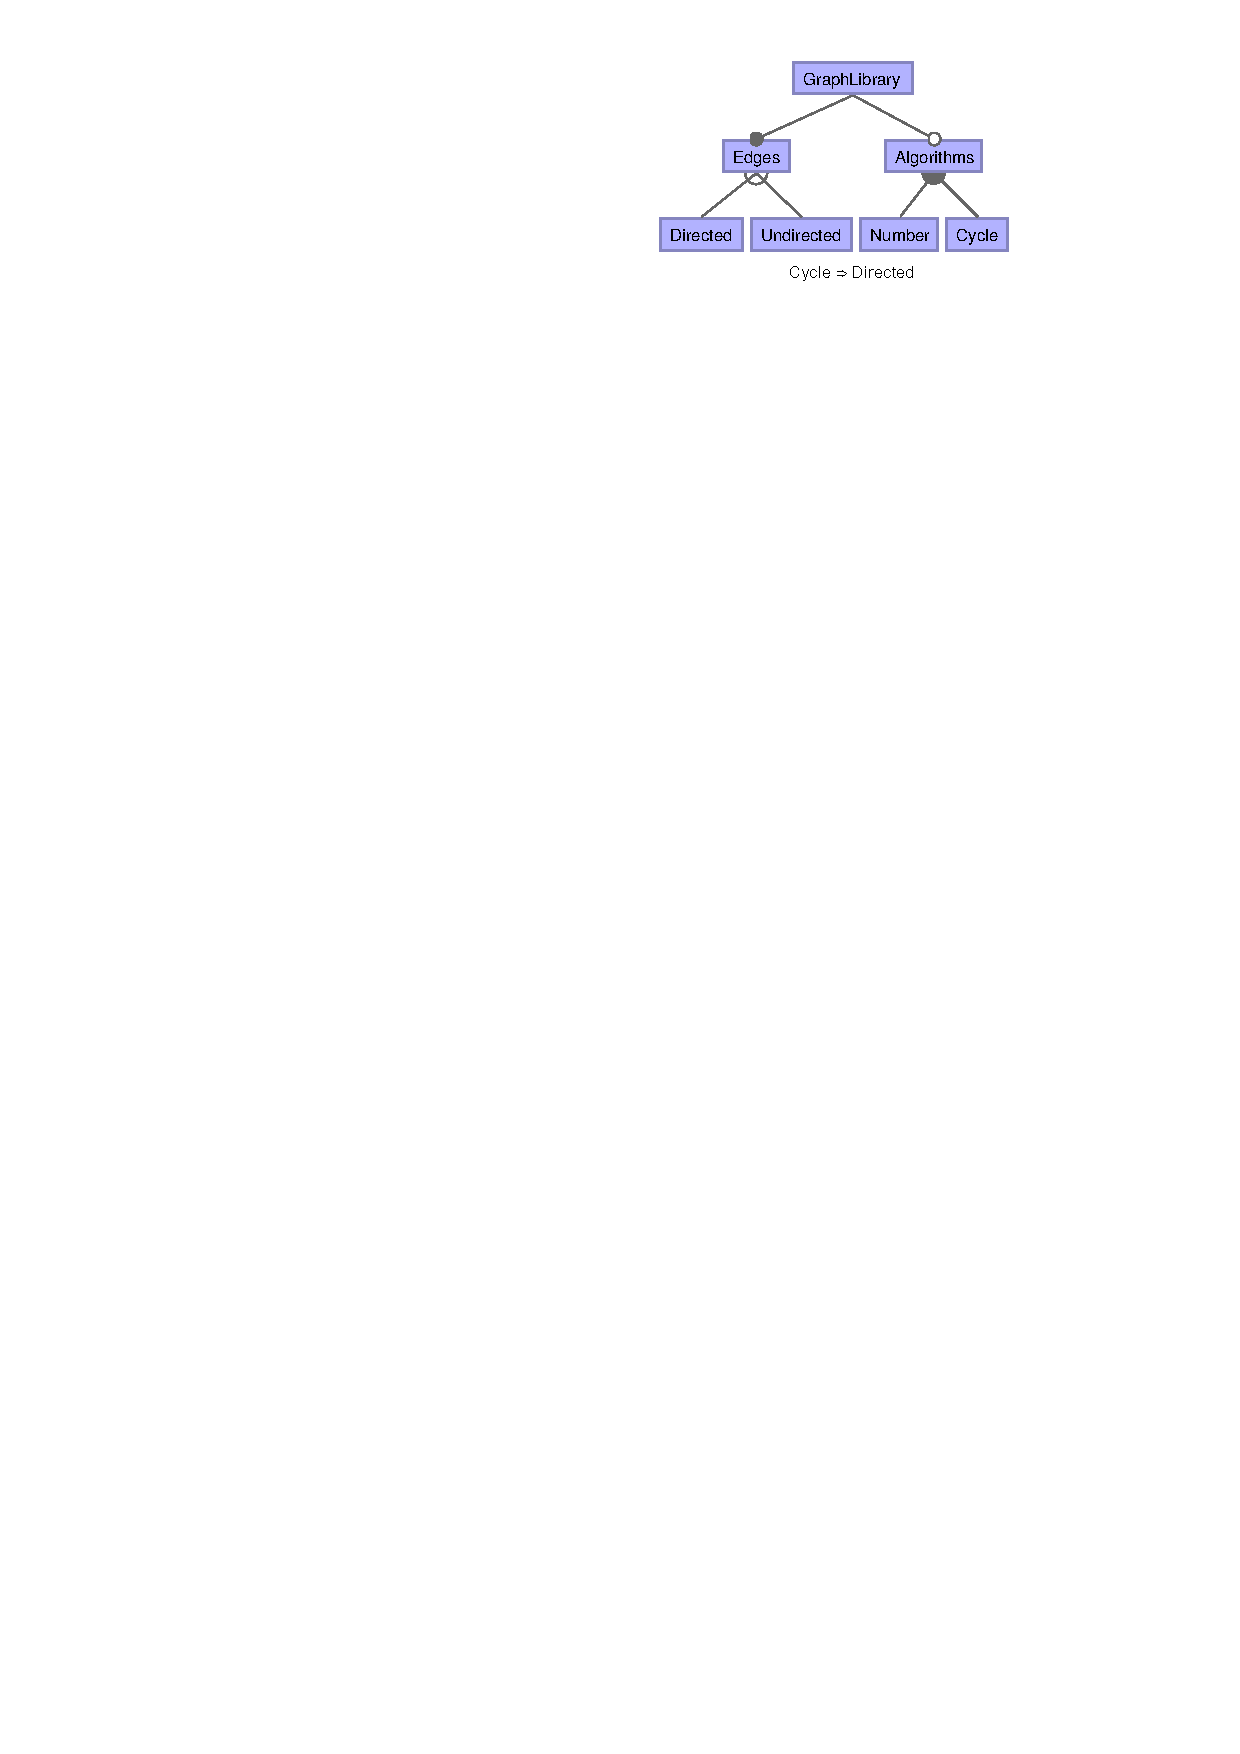
\includegraphics[scale=1.25]{model}
	\caption{A feature model representing a graph product line}
	\label{fig:ex}
\end{figure}

\section{Tables}

\vref{tab:ex} shows the result of a simple tabular environment.

\begin{table}[htbp]
	\centering
		\begin{tabular}{cc}\toprule
			Group Type & Propositional Formula\\\midrule
			And & $(P \pimplies C_{k_1} \wedge\ldots\wedge C_{k_m}) \pand (C_1\vee\ldots\vee C_n \pimplies P)$\\\addlinespace
			Or & $P \pequals C_1\vee\ldots\vee C_n$\\\addlinespace
			Alternative & $(P \pequals C_1\vee\ldots\vee C_n) \pand \mbox{atmost}1(C_1,\ldots,C_n)$\\
			\bottomrule
		\end{tabular}
	\caption{Mapping a feature model to a propositional formula}
	\label{tab:ex}
\end{table}

\section{Code Listings}

In \vref{lst:ex}, we give an example of a source code listing. 

\begin{lstlisting}[style=Java,float=htb,caption={Java source code},label={lst:ex}]
class A extends Object {
	A() { super(); }
}
class B extends Object {
	B() { super(); }
}
class Pair extends Object {
	Object fst;
	Object snd;
	Pair(Object fst, Object snd) {
		super(); this.fst=fst; this.snd=snd;
	}
	Pair setfst(Object newfst) {
		return new Pair(newfst, this.snd);
	}
}
\end{lstlisting}

\chapter{Etablierung Agiler Praktiken}
\label{agilepractices}

% - erkenntnisreichster Teil der Arbeit!
% - Erarbeitung von verwendeten agilen Praktiken
% - Evaluation hinsichtlich ihrer Anwendbarkeit bei den vorher erarbeiteten Problemfeldern

\todots

\section{Methodisches Vorgehen}
\label{agilepractices:methods}

% - genaue Darstellung über Vorgehen in der SLR + Metastudie: 
% - Suchmethodik, Keywords, Kriterien, Auswahlprozes ...
% + Schema der Evaluation (Problemfelder)
% https://docs.google.com/document/d/1j8hegu3FgQk2fPMVjo8IUPWIXwNjlZjT42rHxg7KZ1I/edit

\todots

\section{Literaturübersicht}

% - tabellarische Übersicht, Fallstudien + allgemeine Sekundäre Literatur
% - Inhaltsangabe jeder Arbeit (Zusammenfassung)

\todo{siehe Tabelle 5-7 im Anhang}

\todots

\section{Einsatz agiler Praktiken im Unternehmen}

% - Ergebnisse der SLR - Auflistung der genutzten Methoden

\todo{siehe Tabelle 8  und 9 im Anhang}

\begin{table}[ht]
	\centering
	\caption{Auswertung Nutzung agiler Methoden (kurz)}
	\begin{tabular}{|c|c|}
		\hline
		\textbf{Agile Methode}& \textbf{Anzahl Nennungen} \\
		\hline
		Scrum                          & 17               \\
		Design Thinking                & 10               \\
		DevOps                         & 8                \\
		Kanban                         & 6                \\
		XP                             & 5                \\
		SAFe                           & 4                \\
		Digital Innovation Lab         & 4                \\
		Minimum Valuable Product (MVP) & 2                \\
		Squads and Tribes              & 2                \\
		LeSS                           & 1                \\
		Unified Process                & 1                \\
		Communities of Practice        & 1                \\
		Holacracy                      & 1                \\
		Culture Book                   & 1                \\
		Corporate Startups             & 1                \\
		Agile Modelling                & 1                \\
		Usability Driven Development   & 1                \\
		Lean Startup                   & 1               \\
		\hline
	\end{tabular}
	\label{tab:clusteringagileshort}
\end{table}

\todots

\section{Darstellung und Evaluation verschiedener agiler Methoden}

% - systematisch: erst Definition der Methode, dann Evaluation im Bezug auf die Problemfelder
% - siehe Key findings: https://docs.google.com/document/d/1QayCknP1SgspsPvXlU_FR5u0h2fNzhfQshNOrAuTiB8/edit

\todots

\subsection{Scrum}

\todots

\subsection{Design Thinking}

\todots

\subsection{DevOps}

\todots

\subsection{Kanban}

\todots

\subsection{XP}

\todots

\subsection{SAFe}

\todots

\subsection{Digital Innovation Lab}

\todots

\subsection{Minimum Valuable Product}

\todots

\subsection{Squads and Tribes}

\todots


\section{Formulierung agiler Best-Practice Szenarien}

% - Erstellung von Thesen für Best-Practice Szenarien (im Bezug auf allen Ergebnissen von vorher, vor allen auch 4.3)

\todots



\chapter{Diskussion der Ergebnisse}
\label{evaluation}
%Die Beurteilung ist einer der wichtigsten Abschnitte der Arbeit
%- Sie enthält die Quintessenz des gesamten Projektes
%Viele lesen nur die Einführung und die Beurteilung an
%- Hier muss also alles Wichtige drin stehen!
%Hier beweisen Sie dass Sie …
%- die Aufgabe und deren Bedeutung verstanden haben
%- die Ergebnisse richtig zu interpretieren vermögen
%- wissen, worauf es bei diese Arbeit ankam

% - siehe auch Notizen in: https://docs.google.com/document/d/1jmJIAC5F2cos8MjODSyV-BzwO2jPDtREDRKhCnJRUts/edit#

Das nachfolgende Kapitel soll dazu dienen, dargestellte Ergebnisse kritisch zu evaluieren. Es folgt eine generelle Auseinandersetzung mit der Methodik, möglichen Limitationen bei der Untersuchungen und den eigentlichen Ergebnissen. Darüber hinaus werden mögliche Ansatzpunkte für weiterführende Arbeiten gegeben.

\textbf{Ergebnisse}

Nachfolgend soll eine kritische Betrachtung der vorgestellten Ergebnisse vorgenommen werden. Dafür soll zunächst untersucht werden, inwieweit die in \ref{introduction:fs} dargestellten Forschungsfragen beantwortet werden konnten. 

\hangindent+50pt \hangafter=1
\textbf{Forschungsfrage 1:}\textit{ Wie sehen allgemeine Veränderungsprozesse im Zuge der Digitalen Transformation aus?} Dies wurde in  \ref{problemfields:changepatterns} mittels einer Übersicht, resultierend aus dem SLR 1, vorgenommen. Es hat sich gezeigt, dass es eine große Vielzahl an möglichen Ansatzpunkte für Veränderungen geben kann. Innerhalb der Auswertung hat sich gezeigt, dass eine Clusterung der Nennungen nötig war, da die Begrifflichkeiten teilweise stark voneinander abwichen, die Bedeutung sich jedoch stark ähnelte.  

\hangindent+50pt \hangafter=1
\textbf{Forschungsfrage 2:} \textit{Welche Probleme treten bei der Digitalen Transformation eines Großunternehmens auf?} Auch hierfür wurde eine Übersicht in \ref{problemfields:fields} vorgenommen. Wichtig für die Vergleichbarkeit mit den vorher erarbeiteten Veränderungsprozessmuster war die Gleichheit der zu untersuchenden Literatur in SLR 1. Dies konnte gewährleistet werden. Wiederrum war eine Clusterung der Ergebnisse notwendig.

\hangindent+50pt \hangafter=1
\textbf{Forschungsfrage 3:} \textit{Welche agilen Praktiken bzw. Methoden haben sich in großen Organisationen innerhalb des Transformationsprozesses etabliert?
} Hierfür diente die Durchführung eines zweiten SLR (vgl. \ref{agilepractices:extractions}). Mithilfe einer breiten Auswahl an Literatur, die durch ein bestimmtes Schema ausgewählt wurde, konnte eine große Reihe von agilen Methoden erarbeitet werden, die im Transformationsprozess eingesetzt werden. Wiederrum musste eine Clusterung vorgenommen werden, da teilweise Sonderformen von allgemeinen Methoden eingesetzt wurden. Teilweise war es schwer zu identifizieren, welcher Methode sich bestimmte Prozesse zuordnen lassen können. Unklare Aussagen mussten aussortiert werden, was das Ergebnis unter Umständen verfälscht haben könnte.

\hangindent+50pt \hangafter=1
\textbf{Forschungsfrage 4:} \textit{Wie können agile Praktiken bzw. Methoden dazu beitragen, die vorher erarbeiteten Probleme zu beheben?} Eine vollumfängliche Evaluation mit einem klaren Evaluationsschema und -ziel wurde durchgeführt (vgl. \ref{agilepractices:evaluation}). Hier konnten für fast alle agile Methoden genaue Aussagen für bestimmte Problemfelder identifiziert werden. Innerhalb der Evaluation wurden aus Platzgründen nicht alle in \ref{agilepractices:extractions} aufgeführten Methoden genutzt, sondern nach Wichtigkeit priorisiert, so dass einige aussortiert wurden. Somit hätten weiterführende Evaluationen der restlichen Methoden sicherlich zu einem erweiterten Ergebnis geführt. Die Anzahl der zu bearbeitenden Problemfelder (17 von 21) zeigt aber, dass sich anhand der gewählten agilen Methoden durchaus ein großes Problemspektrum, gerade im Hinblick auf interne Konflikte, lösen lässt. Es hat sich gezeigt, dass sich für die Methode \textit{SAFe} kein positives Evaluationsergebnis erarbeiten lies. Hierfür könnte man durchaus das Auswahlkriterium in \ref{agilepractices:extractions} hinterfragen, in dem Sinne, als dass man eine inhaltliche Auswahl anstatt des Kriteriums der Nennungen hätte wählen können. Nachfolgende Untersuchungen könnten hier durchaus ansetzen, indem man die weiteren Methoden evaluiert. Auch hat die Evaluation ergeben, dass für bestimmte Problemfelde keine Aussagen gefunden werden konnten, obwohl dies durch die Definition der Methode durchaus zutreffend gewesen wäre. Dies ist sicherlich der Tatsache geschuldet, dass in keinen der Fallstudien die Problemfelder explizit untersucht wurden. Ein weiteres Kriterium, welches man hierbei beachten muss, dass die Anzahl der Aussagen mit der Anzahl der Nennungen korrelieren könnten. Beispielsweise ist die Chance auf mehr Aussagen bei der am meisten genannten Methode  \textit{Scrum} viel höher als bei anderen Methoden, da die Menge an verfügbaren Inhalts schlichtweg größer war. 

\hangindent+50pt \hangafter=1
\textbf{Forschungsfrage 5:} \textit{Welche Handlungsmuster lassen sich für einen erfolgreichen Einsatz agiler Praktiken bzw. Methoden im Transformationsprozess ableiten (Best Practices)?}  Hierfür wurden Leitlinien in \ref{agilepractices:bestpractice} aufgestellt. Diese wurden aus den vorhergehenden Ergebnissen abgeleitet, wodurch sie noch nicht als praxistauglich einzustufen sind. Es sind weitere Untersuchungen in diesem Feld nötig, um die erarbeiteten Leitlinien in der Digitalen Transformation zu validieren.

\clearpage

\textbf{Methodik und Limitationen} 

Als übergeordnete Methodik wurde ein zweiteiliges systematisches Literaturreview von Fallstudien (und weiterer Literatur mit Handlungsempfehlungen zur Thematik) vorgenommen. Dies diente dazu, um für beide Hauptteile eine Vielzahl an inhaltlichen Aussagen für die Untersuchungsziele zu generieren, sie zu clustern und zusammenzufassen. Diese Ergebnisse wurden für die Evaluation als Ausgangspunkt genutzt. 

Hinsichtlich der Literatursuche kann gesagt werden, dass die Menge an Ergebnissen in den verschiedenen Suchmaschinen stark variiert hat. Hierbei sollte bei nachfolgenden Untersuchungen in Betracht gezogen werden, die Suche auf bestimmte Suchmaschinen, beispielsweise \textit{Scopus}, einzugrenzen, da sie mehr Ergebnisse erzielten. Darüber hinaus können durchaus andere Suchmaschinen mit anderen, eventuell wirtschaftlicheren Schwerpunkten genutzt werden. Die gewählten Suchmaschinen hatten einen sehr technischen Bezug.

Auch kann die Wahl der Methodik an sich kritisch hinterfragt werden. Innerhalb der Evaluation hätten durchaus andere Formen der Untersuchung gewählt werden können, beispielsweise Beobachtungen, Experteninterviews oder Umfragen. Die Ergebnisse der vorgenommen Evaluation beruhen durchweg aus qualitativen Daten, da nur Aussagen aus der gefundenen Literatur genutzt wurden. Anhand qualitativer Methoden hätten gezieltere Ergebnisse erlangt werden können, da man hier spezifische Untersuchungen zu einzelnen Problemfeldern und agilen Methoden hätte durchführen können. Die Wahl auf das SLR mit abschließender Evaluation erfolgte deshalb, da man sich eine große Menge an bereits verfügbaren Daten versprach. Es wurden vornehmlich Fallstudien zu exakt der Thematik ausgewertet und für weitere Untersuchungen genutzt. Ziel war es, einen gegenwärtigen Status Quo über Problemfelder und Lösungsansätze der Digitalen Transformation zu schaffen und Anreize für nachfolgende Untersuchungen zu schaffen. Anschließend können spezifischere Untersuchungen stattfinden, die sich auf einzelne Problemfelder und agile Methoden beziehen. 

Innerhalb der Untersuchungen traf man auf vereinzelte Limitationen. Nicht alle Fallstudien nannten explizite Problemfelder und eingesetzte agile Methoden. Hierbei konnten nur klare Aussagen verwendet werden. Durch die Aktualität der Thematik Digitale Transformation wird die Menge an zu betrachteten Fallstudien zunehmend größer, so dass auch direkt nach der Untersuchung weitere potenzielle Literatur veröffentlicht wurde, die nicht Eingang in die Ergebnisse fand. Somit haben die vorgenommenen Untersuchungen keinen Anspruch auf Vollständigkeit. Mithilfe der Einschlusskriterien in beiden SLR wurde versucht,  die Auswahl einzugrenzen.

\textbf{Nachfolgende Arbeiten} 

Wie bereits aufgeführt, bilden die Ergebnisse Ansatzpunkte für nachfolgende Untersuchungen. Mithilfe von genauen Beobachtungen kann validiert werden, ob sich die Problemfelder tatsächlich mit den verlinkten agilen Methoden bearbeiten lassen (vgl. \ref{tab:clusteringfinal}). Des Weiteren sollten die Leitlinien mithilfe weiterer Untersuchungen validiert werden. Ein Kriterium, welches in der vorliegenden Arbeit nicht betrachtet wurde, sind mögliche kulturelle Unterschiede in einzelnen Unternehmen durch verschiedene Nationalitäten. In der Auswahl der Herkunft der Großunternehmen wurden keine Abgrenzungen vorgenommen. Sicherlich sollte untersucht werden, wie gerade bei der Konfliktlösung solche kulturellen Werte verschiedener Mitarbeitergruppen betrachtet werden können. Bestimmte agile Methoden, beispielsweise Design Thinking, bilden bereits erste Ansätze. Die Digitale Transformation bietet ein breites Feld für genaue Untersuchungen, gerade hinsichtlich den mit ihr einhergehenden Veränderungsprozessen.
\chapter{Zusammenfassung}
\label{conclusion}

Das übergeordnete Ziel der vorliegenden Arbeit sollte die Evaluation verschiedener agiler Methoden als mögliche Change Management Instrumente innerhalb der Digitalen Transformation von Großunternehmen sein. Es wurden beispielhafte Leitlinien herausgearbeitet, die zeigen, in welcher Art und Weise Agilität im Allgemeinen und agile Werte im Besonderen in Veränderungsprozessen eingesetzt werden können.

Als erster Schwerpunkt konnten eine Reihe von Veränderungsprozessmuster in der Digitalen Transformation mittels eines systematischen Literaturreviews erarbeitet werden (vgl. \ref{problemfields}). Diese zeigen, in welchen Bereichen Veränderungen entstehen können. Darüber hinaus wurden insgesamt 21 Problemfelder der Digitalen Transformation identifiziert. Diese zeigen durch die Analyse von mehreren Fallstudien einen aktuellen Status Quo, in welchen Bereichen es vermehrt zu Problemen in den Veränderungsprozessen gekommen ist. Beispielsweise hat sich gezeigt, dass es gegenwärtig starke Probleme in der Kundenorientierung der Produktentwicklung gibt. Teilweise fehlte diese komplett.

Die erarbeiteten Problemfelder bildeten die Grundlage für die nachfolgende Evaluation agiler Methoden im Kontext der Digitalen Transformation (vgl.  \ref{agilepractices}). Dafür wurde zunächst ein weiteres SLR durchgeführt, um eine Reihe agiler Methoden zu extrahieren, die vermehrt im Transformationsprozess eingesetzt werden. Anschließend wurden in einer systematischen Evaluation 9 ausgewählte Methoden hinsichtlich ihrer Anwendbarkeit in bestimmten Problemfelder untersucht. Es hat sich gezeigt, dass die Ansatzpunkte sehr unterschiedlich und durchaus vielversprechend sind. Beispielsweise hat sich Scrum als sehr effektiv gezeigt, in dem es durch seine agile Werte in vielen Problemfeldern eingesetzt werden kann. Es hat sich gezeigt, dass vor allem durch die Mischung verschiedener agiler Ansätze große Erfolgschancen erreichbar sind.

Die erarbeiteten Leitlinien können als Ausgangspunkt für erfolgreiche Implementationen agiler Methodiken in der Digitalen Transformation genutzt werden. Es hat sich gezeigt, dass die Ergebnisse einen sehr allgemeinen Überblick über den Einsatz verschiedener agiler Methoden bieten. Nachfolgende Untersuchungen haben die Chance, agile Methoden in speziellen Problemszenarien zu beobachten. So kann gezeigt werden, inwieweit die Ergebnisse, die zunächst auf spezifische Aussagen aus bereits vorhandenen Fallstudien basieren, in der Praxis umgesetzt werden können. 

Die Digitale Transformation ist ein Prozess, der aktuell eine sehr hohe Bedeutung genießt, und dessen noch eher junger Forschungsstand ein großen Raum für neue Erkenntnisse bietet. Die vorliegende Arbeit hat unter anderem auch gezeigt, dass der Prozess mit vielen Problemen behaftet sein kann, er aber dennoch in der Agenda eines jeden Großunternehmens verankert sein sollte, um mit neuen, digitalen Produktangeboten konkurrenzfähig zu bleiben.
%\ifgerman{\chapter{Zukunftige Arbeiten}}{\chapter{Future Work}}
\label{futurework}

\todots

%*********************************************************************%
% APPENDIX                                                            %
%*********************************************************************%

\appendix
\ifgerman{\chapter{Anhang}}{\chapter{Appendix}}
\label{appedixa}

\begin{table}[ht]
	\caption{Literaturübersicht SLR 1 Problemfelder (Teil 1)}
	\centering
	\begin{tabularx}{500px}{|X|X|X|}
		\hline
		\textbf{Referenz}                                            & \textbf{Titel}                                                                                                                                                                   & \textbf{Untersuchungsgegenstand}                                                                                                                                         \\
		\hline
		\citeA{muchna_aspekte_2018} (1)                                  & Aspekte des Innovations- und Changemanagements. Ein Theorie-Praxis-Transfer                                                                                              & 1 Fallstudie zum Deutschen Bankensektor                                                                                                                         \\
		\citeA{gassmann_digitale_2016} (2)                & Digitale Transformation im Unternehmen gestalten: Geschäftsmodelle Erfolgsfaktoren Fallstudien                                                                           & 11 Fallstudien zu Großunternehmen im deutschsprachigen Raum                                                                                                     \\
		\citeA{chanias_digital_2018} (3)        & Digital transformation strategy making in pre-digital organizations: The case of a financial services provider                                                           & 1 Fallstudie einen Unternehmen aus dem Finanzsektor, anonymisiert                                                                                               \\
		\citeA{urbach_digitalization_2018} (4)               & Digitalization Cases How Organizations Rethink Their Business for the Digital Age                                                                                        & 21 Fallstudien von Großunternehmen                                                                                                                              \\
		\citeA{gartner_fallstudien_2018}  (5)              & Fallstudien zur Digitalen Transformation: Case Studies für die Lehre und praktische Anwendung                                                                            & 9 Fallstudien zur Digitalisierung, international                                                                                                                \\
		\citeA{oswald_digitale_2018}  (6)                  & Digitale Transformation: Fallbeispiele und Branchenanalysen                                                                                                              & 4 Fallstudien im deutschsprachigen Raum, darunter insgesamt 59 Unternehmen aus verschiedenen Bereichen + Daten aus 650 Organisationen in der Automobilindustrie \\
		\citeA{hoberg_skills_2017}  (7)                                & Skills for Digital Transformation                                                                                                                                        & 1 Studie mit 116 Vertretern aus Konzernen aus 18 verschiedenen Ländern                                                                                          \\
		\citeA{solis_2017_2017}  (8)               & The 2017 State of Digital Transformation                                                                                                                                 & 1 Studie mit 528 Offizielen aus Großunternehmen weltweit                                                                                                        \\
		\citeA{kremins_2018_2018} (9)                             & The 2018 Digital Transformation report                                                                                                                                   & 1 Studie mit 200 Offizielen aus der internationen Reisebranche                                                                                                  \\
		\citeA{heinemann_digitale_2016} (10) & Digitale Transformation oder digitale Disruption im Handel                                                                                                               & 15 Fallstudien aus der Handelsbranche, international                                                                                                            \\
		\citeA{nowik_promoting_2018}  (11)                                & Promoting Digital Transformation in Digitally Developing Industries - A case study on strategic action points driving digital transformation in the real estate industry & 1 Studie mit Offizielen aus verschieden schwedischen Firmen in der Immobilienbranche                                                                            \\
		\citeA{buhse_transformationswerk_2016}  (12)                 & Transformationswerk Report 2016                                                                                                                                          & 1 Studie mit 1.060 Vertretern aus Konzernen und dem Mittelstand                                                                                                 \\
		\citeA{wautelet_impact_2017}  (13)                              & The impact of digitalization on international companies: a case study of LEGO                                                                                            & 1 Fallstudie eines Großunternehmens                                                                                                                             \\
		\hline                                                                                          
	\end{tabularx}
	\label{tab:overviewliterature1}
\end{table}

\begin{table}[ht]
	\caption{Literaturübersicht SLR 1 Problemfelder (Teil 2)}
	\centering
	\begin{tabularx}{500px}{|X|X|X|}
		\hline
		\textbf{Referenz}                                            & \textbf{Titel}                                                                                                                                                                   & \textbf{Untersuchungsgegenstand}                                                                                                                                         \\
		\hline
		\citeA{weber_digital_2015}   (14)                                & Digital Navigator. Handlungsfelder der digitalen Transformation und Stand der Digitalisierung im deutschsprachigen Raum                                                  & 82 Fallstudien von Unternehmen aus IKT-Sektor                                                                                                                   \\
		\citeA{hess_options_2016}  (15)                                   & Options for Formulating a Digital Transformation Strategy                                                                                                                & 3 Fallstudien von großen Medienkonzerne aus dem deutschsprachigen Raum                                                                                          \\
		\citeA{depiereux_studie_2018}  (16)                              & Studie Digitale Transformation 2018 Hemmnisse, Fortschritte, Perspektiven                                                                                                & 1 Studie von 2.000 deutschen Großunternehmen                                                                                                                    \\
		\citeA{buxmann_digitalisieren_2016}  (17)               & Digitalisieren Sie schon? Ein Benchmark für die digitale Agenda                                                                                                          & 1 Studie mit 103 Unternehmen aus den Branchen Industrie/Maschinen- und Anlagenbau, Automotive sowie Logistik/Transport                                          \\
		\citeA{berghaus_2016}  (18)                & Wie packen Unternehmen die digitale Transformation an? Ratgeber und Fallstudien zur Strategiearbeit für das digitale Zeitalter                                           & 5  Fallstudien von Großunternehmen im deutschsprachigen Raum                                                                                                    \\
		\citeA{kawohl_digitale_2016} (19)                   & Digitale Transformation: Wie weit sind die DAX 30?                                                                                                                       & 30 Fallstudien der DAX-Unternehmen                                                                                                                              \\
		\citeA{beule_digital_2019} (20)   & Digital Transformation of Radio Broadcasting: An Exploratory Analysis of Challenges and Solutions for New Digital Radio Services                                         & 6 Fallstudien aus der internationalen Radio-Branche                                                                                                             \\
		\citeA{oswald_shaping_2017}   (21)          & Shaping the Digital Enterprise Trends and Use Cases in Digital Innovation and Transformation                                                                             & 3 Fallstudien von Großunternehmen                                                                                                                               \\
		\citeA{savastano_how_2018}   (22)                          & How Digital Transformation is Reshaping the Manufacturing Industry Value Chain: The New Digital Manufacturing Ecosystem Applied to a Case Study from the Food Industry   & 1 Fallstudie aus der Ernährungsbranche                                                                                                                          \\
		\citeA{macgillavry_digital_2014}  (23)               & Digital Transformation at DHL Freight: The Case of a Global Logistics Provider                                                                                           & 1 Fallstudie eines Großunternehmen aus der Logistikbranche          \\
		\hline                                                                            
	\end{tabularx}
	\label{tab:overviewliterature1-2}
\end{table} 

\begin{sidewaystable}[ht]
	\centering
	\caption[Auswertung SLR 1 Veränderungsprozessmuster]{Auswertung SLR 1 Veränderungsprozessmuster \protect \footnotemark}
	\begin{tabular}{|p{6cm}|c|c|c|c|c|c|c|c|c|c|c|c|c|c|c|c|c|c|c|c|c|c|c|c|c|}
		\hline
		& 1 & 2 & 3 & 4 & 5 & 6 & 7 & 8 & 9 & 10 & 11 & 12 & 13 & 14 & 15 & 16 & 17  & 18 & 19 & 20 & 21 & 22 & 23 & $\sum$  \\
		\hline
		Einführung einer Multi-Kanal-Strategie              & x                 &                    &                    & x                    &                    & x                 &                   & x                    &                    & x                    &                  &                  & x                   &                  &                 &                      &                    &                 &                  &                  &                        &                      &                        & 6  \\
		Wechsel vom Offline- zum Online-Vertrieb            & x                 &                    &                    &                      &                    &                   &                   & x                    &                    & x                    &                  &                  &                     &                  &                 &                      & x                  &                 &                  &                  &                        & x                    &                        & 5  \\
		Erschaffung neuer digitaler Produkte                & x                 &                    & x                  & x                    & x                  &                   &                   &                      &                    & x                    &                  & x                & x                   & x                &                 &                      & x                  &                 & x                &                  & x                      &                      & x                      & 12 \\
		Tendenz zur Kundenorientierung                      &                   & x                  & x                  & x                    &                    & x                 & x                 & x                    & x                  & x                    & x                & x                & x                   & x                &                 & x                    & x                  &                 & x                &                  &                        & x                    &                        & 16 \\
		Digitalisierung des Geschäftsmodells     &                   & x                  & x                  & x                    & x                  & x                 & x                 &                      &                    & x                    &                  & x                & x                   &                  & x               &                      &                    &                 &                  &                  &                        &                      & x                      & 11 \\
		Digitaler Wissensaufbau im Unternehmen              &                   & x                  &                    & x                    &                    & x                 &                   &                      &                    & x                    & x                & x                &                     & x                &                 & x                    & x                  &                 & x                & x                & x                      &                      &                        & 12 \\
		Datengestützte Verbesserungsprozesse    &                   & x                  &                    & x                    & x                  &                   &                   &                      &                    &                      & x                &                  &                     &                  &                 &                      &                    &                 &                  & x                &                        &                      &                        & 5  \\
		Erzeugung eines digitalen Ökosystems &                   & x                  &                    & x                    &                    & x                 &                   & x                    &                    & x                    & x                &                  &                     &                  &                 &                      & x                  &                 &                  &                  &                        &                      &                        & 7  \\
		Digitalisierung von internen Prozessen              &                   & x                  &                    & x                    &                    & x                 &                   &                      & x                  & x                    &                  &                  &                     &                  & x               &                      &                    &                 &                  &                  &                        & x                    &                        & 7  \\
		Einbindung innovativer Technologien                 &                   &                    &                    & x                    & x                  & x                 &                   &                      & x                  &                      &                  &                  &                     &                  & x               &                      &                    &                 &                  &                  & x                      &                      &                        & 6  \\
		Aufbau technisches Sicherheitskonzept      &                   &                    &                    & x                    &                    &                   &                   & x                    &                    &                      &                  &                  &                     & x                &                 &                      &                    & x               &                  &                  &                        &                      &                        & 4  \\
		Digitale Neuausrichtung der Organisation            &                   & x                  &                    & x                    &                    & x                 &                   & x                    & x                  & x                    &                  &                  &                     & x                & x               & x                    &                    & x               & x                &                  & x                      &                      & x                      & 13 \\
		Innovationsförderung                                &                   &                    &                    &                      &                    &                   &                   & x                    &                    & x                    &                  &                  & x                   & x                &                 & x                    & x                  & x               &                  &                  &                        &                      &                        & 7  \\
		Kooperation mit externen Treibern                   &                   & x                  &                    &                      &                    &                   &                   &                      &                    & x                    &                  &                  &                     & x                &                 & x                    & x                  &                 &                  &                  &                        &                      &                        & 5 \\
		\hline
	\end{tabular}
	\label{tab:clusteringchangeprocess}
\end{sidewaystable}
\footnotetext{Nummerierungen sind der \ref{tab:overviewliterature1} und \ref{tab:overviewliterature1-2} zu entnehmen}

\begin{sidewaystable}[ht]
	\centering
	\caption[Auswertung SLR 1 Problemfelder]{Auswertung SLR 1 Problemfelder \protect \footnotemark}
	\begin{tabular}{|p{6cm}|c|c|c|c|c|c|c|c|c|c|c|c|c|c|c|c|c|c|c|c|c|c|c|c|c|}
		\hline
		& 1 & 2 & 3 & 4 & 5 & 6 & 7 & 8 & 9 & 10 & 11 & 12 & 13 & 14 & 15 & 16 & 17 & 18 & 19 & 20 & 21 & 22 & 23 & $\sum$  \\
		\hline
		Unternehmensweite Kommunikationsprobleme        & x                 & x                  &                    & x                    & x                  &                   &                   &                      &                    &                      &                  &                  &                     &                  &                 &                      & x                  &                 &                  &                  &                        &                      &                        & 5  \\
		Festhalten an verfestigten Strukturen           & x                 & x                  &                    & x                    &                    &                   &                   & x                    &                    &                      & x                &                  &                     &                  &                 & x                    &                    & x               &                  &                  &                        &                      &                        & 7  \\
		Zeit - und Marktdruck                           & x                 &                    &                    & x                    & x                  &                   &                   &                      &                    &                      &                  & x                &                     &                  &                 & x                    &                    &                 &                  &                  &                        &                      &                        & 5  \\
		Unterschätzung der Komplexität                  & x                 &                    &                    & x                    & x                  &                   & x                 &                      &                    &                      &                  &                  &                     &                  &                 &                      &                    &                 &                  &                  &                        &                      &                        & 4  \\
		Fehlende Kontinuierliche Verbesserungsprozesse  &                   & x                  & x                  & x                    &                    &                   &                   &                      &                    & x                    &                  &                  &                     & x                &                 &                      &                    &                 &                  &                  &                        & x                    & x                      & 7  \\
		Störung durch oberes Management (Top-Down)      &                   & x                  & x                  & x                    &                    &                   &                   & x                    &                    & x                    &                  &                  &                     &                  &                 &                      & x                  & x               &                  &                  &                        &                      &                        & 7  \\
		Konflikte zwischen IT und Business              &                   & x                  &                    & x                    &                    & x                 &                   &                      &                    &                      &                  &                  &                     &                  &                 &                      & x                  &                 &                  &                  &                        &                      &                        & 4  \\
		Fehlende frühe Einbeziehung aller Mitarbeiter   &                   & x                  &                    & x                    &                    &                   &                   &                      &                    &                      &                  &                  &                     &                  &                 &                      &                    &                 & x                &                  &                        &                      &                        & 3  \\
		Sicherheitsprobleme                             &                   &                    &                    & x                    &                    & x                 &                   &                      &                    &                      &                  &                  &                     &                  &                 &                      &                    &                 &                  &                  &                        &                      &                        & 2  \\
		Fehlende Kundenorientierung                     &                   & x                  &                    & x                    & x                  & x                 &                   & x                    & x                  & x                    & x                &                  & x                   &                  &                 & x                    &                    &                 & x                & x                & x                      &                      &                        & 13 \\
		Fehlendes technischen Know-How                  &                   & x                  &                    & x                    &                    & x                 & x                 & x                    &                    & x                    &                  & x                &                     & x                &                 &                      &                    &                 & x                &                  &                        &                      & x                      & 10 \\
		Fehlende monetäre Ressourcen                    &                   &                    &                    & x                    &                    &                   &                   & x                    &                    &                      &                  &                  &                     &                  &                 &                      &                    &                 &                  &                  &                        &                      &                        & 2  \\
		Rechtliche Bestimmungen und Datenschutz         &                   &                    &                    & x                    &                    & x                 &                   &                      &                    & x                    &                  &                  &                     &                  &                 & x                    &                    &                 &                  & x                &                        &                      &                        & 5  \\
		Fehlende Transparenz (intern und extern)        &                   &                    &                    & x                    & x                  & x                 &                   &                      &                    & x                    &                  &                  &                     &                  &                 &                      &                    &                 &                  &                  &                        &                      &                        & 4  \\
		Fehlende Partnerschaften                        &                   & x                  &                    & x                    &                    & x                 &                   &                      &                    & x                    & x                &                  &                     & x                &                 &                      &                    &                 &                  &                  &                        &                      &                        & 6  \\
		Fehlende Innovationskultur                      &                   & x                  &                    & x                    & x                  &                   &                   &                      &                    & x                    &                  &                  &                     & x                &                 &                      &                    &                 &                  &                  &                        &                      & x                      & 6  \\
		Langsame Entscheidungsprozesse                  &                   &                    &                    & x                    &                    &                   &                   &                      &                    & x                    &                  &                  &                     &                  &                 & x                    &                    &                 &                  &                  &                        &                      &                        & 3  \\
		Unternehmenskulturelle Probleme                 &                   & x                  &                    & x                    & x                  & x                 &                   &                      & x                  & x                    &                  & x                &                     &                  & x               &                      &                    &                 &                  &                  &                        &                      &                        & 8  \\
		Fehlendes Vertrauen, Akzeptanz und Bereitschaft &                   &                    &                    & x                    & x                  &                   &                   &                      &                    & x                    & x                & x                &                     &                  &                 & x                    &                    & x               &                  &                  & x                      &                      & x                      & 9  \\
		Unklare Verantwortlichkeiten                    &                   & x                  &                    & x                    & x                  &                   & x                 &                      &                    &                      &                  & x                &                     &                  &                 &                      &                    &                 &                  &                  &                        &                      &                        & 5  \\
		Fehlende digitale Strategie                     &                   & x                  &                    &                      &                    & x                 & x                 &                      &                    & x                    &                  & x                &                     &                  &                 &                      &                    &                 &                  &                  & x                      &                      &                        & 6 \\
		\hline
	\end{tabular}
	\label{tab:clusteringproblemfields}
\end{sidewaystable}
\footnotetext{Nummerierungen sind der \ref{tab:overviewliterature1} und \ref{tab:overviewliterature1-2} zu entnehmen}

\begin{table}[ht]
	\caption{Literaturübersicht SLR 2 Agile Methoden (Teil 1)}
	\centering
	\begin{tabularx}{500px}{|X|X|X|}
		\hline
		\textbf{Referenz}                                            & \textbf{Titel}                                                                                                                                                                   & \textbf{Untersuchungsgegenstand}                                                                                                                                         \\
		\hline
		\citeA{fuchs_adapting_2019} (1)                                   & Adapting (to) Agile Methods: Exploring the Interplay of Agile Methods and Organizational Features                                             & 4 Fallstudien aus Großunternehmen, anonymisiert                                                             \\
		\citeA{prasad_adopting_2018} (2)     & Adopting Design Thinking Practices to Satisfy Customer Expectations in Agile Practices: A Case from Sri Lankan Software Development Industry  & 10 Fallstudien in IT Service Organisationen                                                                 \\
		\citeA{alawairdhi_agile_2016} (3)                              & Agile development as a change management approach in software projects: Applied case study                                                    & 2 Softwareprojekte an der Electronic University Saudi-Arabien                                               \\
		\citeA{mikalsen_agile_2018} (4)                              & Agile Digital Transformation: A Case Study of Interdependencies                                                                               & 1 Fallstudie aus dem Bankenwesen                                                                            \\
		\citeA{looks_agile_2018} (5)  & Agile Projekte in öffentlichen Verwaltungen - Eine Bestandsaufnahme                                                                           & 1 Umfrage an 38 Personen aus der öffentlichen Verwaltung                                                    \\
		\citeA{kilu_agile_2019} (6)                                & Agile Software Process Improvement by Learning from Financial and Fintech Companies: LHV Bank Case Study                                      & 1 Fallstudie aus dem Bankenwesen + 4 Interviews mit 4 Unternehmen aus dem Bankenwesen                       \\
		\citeA{drilling_agilitat_nodate} (7)               & Agilität und DevOps fördern digitale Transformation                                                                                           & 1 Studie mit 1770 Senior Business- und IT-Entscheider aus 21 Ländern und 10 verschiedenen Industriebranchen \\
		\citeA{dikert_challenges_2016} (8) & Challenges and success factors for large-scale agile transformations: A systematic literature review                                          & 52 Publikationen über 42 Fallstudien aus verschiedenen Industrien                                           \\
		\citeA{paasivaara_communities_2014} (9)        & Communities of practice in a large distributed agile software development organization – Case Ericsson                                        & 1 Fallstudie                                                                                                \\
		\citeA{chanias_digital_2018} (10)         & Digital transformation strategy making in pre-digital organizations: The case of a financial services provider                                & 1 Fallstudie einen Unternehmen aus dem Finanzsektor, anonymisiert                                           \\
		\citeA{heinemann_digitale_2016} (11) & Digitale Transformation oder digitale Disruption im Handel                                                                                    & 15 Fallstudien aus der Handelsbranche, international                                                        \\
		\citeA{urbach_digitalization_2018} (12)                & Digitalization Cases How Organizations Rethink Their Business for the Digital Age                                                             & 21 Fallstudien Großunternehmen weltweit                                                                     \\
		\hline                                                                                          
	\end{tabularx}
	\label{tab:overviewliterature2}
\end{table}

\begin{table}[ht]
	\caption{Literaturübersicht SLR 2 Agile Methoden (Teil 2)}
	\centering
	\begin{tabularx}{500px}{|X|X|X|}
		\hline
		\textbf{Referenz}                                            & \textbf{Titel}                                                                                                                                                                   & \textbf{Untersuchungsgegenstand}                                                                                                                                         \\
		\hline
		\citeA{mihelic_embracing_nodate} (13)                                 & Embracing Design Thinking in medium-sized enterprises                                                                                         & 1 Erfahrungsbericht eines Unternehmens                                                                      \\
		\citeA{gerster_how_2019} (14)                                & How Enterprises Adopt Agile Structures: A Multiple-Case Study                                                                                 & 12 Fallstudien von internationen Unternehmen                                                                \\
		\citeA{anwar_agile_2016} (15)          & Agile Adoption Case Study, Pains, Challenges \& Benefits                                                                                      & 1 Fallstudie eines Entwicklungsteams innerhalb eines Großunternehmens                                       \\
		\citeA{wiedemann_implementing_2019} (16)                              & Implementing the Planning Process within DevOps Teams to Achieve Continuous Innovation                                                        & 23 Interviews mit Vertretern (CTO, IT Manager ..) aus deutschen Großunternehmen                             \\
		\citeA{paasivaara_large-scale_2018} (17)                             & Large-scale agile transformation at Ericsson: a case study                                                                                    & 1 Fallstudie                                                                                                \\
		\citeA{weinreich_lean_2016} (18)                              & Lean Digitization - Digitale Transformation durch agiles Management                                                                           & Keine Fallstudie, aber strukturierte Handlungsempfehlungen                                                  \\
		\citeA{somsen_rerouting_2019} (19)                                & Rerouting Digital Transformations                                                                                                             & 6 Fallstudien aus der Flugbranche                                                                           \\
		\citeA{oswald_shaping_2017} (20)            & Shaping the Digital Enterprise Trends and Use Cases in Digital Innovation and Transformation                                                  & 3 Fallstudien von Großunternehmen                                                                           \\
		\citeA{shahzad_training_nodate} (21)       & Training for Agile Transformation at Universities: A Case Study Analysis                                                                      & 1 Fallstudie, Agiles Training an einer staatlichen Universität                                              \\
		\citeA{berghaus_2016} (22)                  & Wie packen Unternehmen die digitale Transformation an? Ratgeber und Fallstudien zur Strategiearbeit für das digitale Zeitalter                & 5 Fallstudien mit Großunternehmen im deutschsprachigen Raum                                                 \\
		\citeA{gassmann_digitale_2016} (23)               & Digitale Transformation im Unternehmen gestalten: Geschäftsmodelle Erfolgsfaktoren Fallstudien                                                & 11 Großunternehmen im deutschsprachigen Raum                                                                \\
		\citeA{gurusamy_integrated_2016} (24)                               & An Integrated Framework for Design Thinking and Agile Methods for Digital Transformation                                                      & Keine Fallstudie, aber Handlungsempfehlungen                                                                \\
		\citeA{klunder_becoming_2018} (25)     & Becoming Agile while preserving software product lines: an Agile transformation model for large companies                                     & Keine Fallstudie, aber Handlungsempfehlungen                                                                \\
		\citeA{laanti_agile_2017} (26)                                  & Agile transformation model for large software development organizations                                                                       & 1 Fallstudie eines Großunternehmens aus der Finanzbranche                                                   \\
		\hline                                                                                          
	\end{tabularx}
	\label{tab:overviewliterature2-2}
\end{table}

\begin{table}[ht]
	\caption{Literaturübersicht SLR 2 Agile Methoden (Teil 3)}
	\centering
	\begin{tabularx}{500px}{|X|X|X|}
		\hline
		\textbf{Referenz}                                            & \textbf{Titel}                                                                                                                                                                   & \textbf{Untersuchungsgegenstand}                                                                                                                                         \\
		\hline
		\citeA{komus_status_2017} (27)                   & Status Quo Agile Studie zu Verbreitung und Nutzen agiler Methoden Eine empirische Untersuchung                                                & 1 Studie mit über 1.000 Teilnehmer aus über 30 Ländern                                                    \\
		\citeA{hofert_agile_2018} (28)                                  & Das agile Mindset                                                                                                                             & 4 Fallstudien aus dem deutschen Raum                                                                        \\
		\citeA{alt_innovationsorientiertes_2017} (29)           & Innovationsorientiertes IT-Management mit DevOps: IT im Zeitalter von Digitalisierung und Software-defined Business                           & 1 Fallstudie eines Großunternehmens                                                                         \\
		\citeA{rodriguez_combining_2014} (30)                              & Combining Lean Thinking and Agile Methods for Software Development: A Case Study of a Finnish Provider of Wireless Embedded Systems Detailed  & 1 Fallstudie eines Großunternehmens                                                                         \\
		\citeA{alahyari_exploratory_2019} (31) & An exploratory study of waste in software development organizations using agile or lean approaches: A multiple case study at 14 organizations & 14 Fallstudien von Großunternehmen                                                                          \\
		\citeA{eklund_scaling_2017} (32)                & Scaling agile development in mechatronic organizations - a comparative case study                                                             & 1 Fallstudie in der Mechatronischen Industrie   \\
		\hline                                                                                          
	\end{tabularx}
	\label{tab:overviewliterature2-3}
\end{table}

\begin{sidewaystable}[ht]
	\centering
	\caption[Auswertung SLR 2 agile Methoden (Teil 1)]{Auswertung SLR 2 agile Methoden (Teil 1) \protect \footnotemark}
	\begin{tabular}{|l|p{8cm}|p{8cm}|}
		\hline
		\textbf{Referenz}                                            & \textbf{Anwendungsgebiet}                                                                                                &\textbf{agile Methoden}                                                                       \\
		\hline                                                               
		(1)                                  & Innovationsmanagement                                                                                              & Scrum, SAFe, LeSS, Kanban                                                                        \\
		(2)     & kundenzentrierte Produktentwicklung                                                                                & Design Thinking                                                                                  \\
		(3)                            & Produktentwicklung                                                                                                 & Scrum                                                                                            \\
		(4)                               & kundenzentrierte Produktentwicklung                                                                                & Scrum, DevOps (BizDev)                                                                           \\
		(5) & agile Organisationsentwicklung & Scrum \\
		(6)                                    & Produktentwicklung                                                                                                 & Scrum, Kanban, XP                                                                                \\
		(7)                & agile Organisationsentwicklung                                                                                     & DevOps                                                                                           \\
		(8) & Produktentwicklung                                                                                                 & Scrum, Unified Process, Extreme Programming, Kanban                                              \\
		(9)           & Produktentwicklung, Kontinuierliche Verbesserungsprozesse                                                          & Scrum, Communities of Practice                                                                   \\
		(10)          & Produktentwicklung                                                                                                 & Minimum Viable Product (MVP)                                                                   \\
		(11) & agile Organisationsentwicklung, Produktentwicklung                                                                 & Holacracy, Culture Book, Squads and Tribes, Scrum                                                \\
		(12)                                & Innovationsmanagement                                                                                              & Design Thinking                                                                                  \\
		(13)                                & agile Organisationsentwicklung                                                                                     & Squads and Tribes                                                                                \\
		(14)          & Produktentwicklung                                                                                                 & Scrum                                                                                            \\
		(15)              & Prozessautomatisierung, kundenzentrierte Produktentwicklung, Innovationsmanagement, agile Organisationsentwicklung & Scrum, Digital Innovation Lab, DevOps, Design Thinking, SAFe                                     \\
		(16)                            & Innovationsmanagement, kundenzentrierte Produktentwicklung                                                         & DevOps                                                                                           \\
		(17)                              & Produktentwicklung                                                                                                 & Scrum                                                                                            \\
		(18)                               & Agile Organisation, Produktentwicklung, Innovationsmanagement                                                      & Design Thinking, Digital Innovation Lab, Corporate Startups, DevOps                              \\
		(19)                                  & Agile Organisation                                                                                                 & Scrum                                                                                            \\
		(20)             & Produktentwicklung, Innovationsmanagement                                                                          & Design Thinking, Digital Innovation Lab                                                          \\
		(21)        & Wissensmanagement                                                                                                  & XP                                                                                               \\
		(22)                  & Digitale Strategie                                                                                                 & Design Thinking, Digital Innovation Lab                                                          \\
		(23)                  & Produktentwicklung                                                                                                 & Design Thinking, Minimum Viable Product (MVP)                                                  \\
		\hline
	\end{tabular}
	\label{tab:clusteringslr2}
\end{sidewaystable}
\footnotetext{Nummerierungen sind der \ref{tab:overviewliterature2}, \ref{tab:overviewliterature2-2} und \ref{tab:overviewliterature2-3} zu entnehmen}

\begin{sidewaystable}[ht]
	\centering
	\caption[Auswertung SLR 2 agile Methoden (Teil 2)]{Auswertung SLR 2 agile Methoden (Teil 2) \protect \footnotemark}
	\begin{tabular}{|l|p{8cm}|p{8cm}|}
		\hline
		\textbf{Referenz}                                            & \textbf{Anwendungsgebiet}                                                                                                &\textbf{agile Methoden}                                                                       \\
		\hline
		(24)                                & Produktentwicklung                                                                                                 & XP, Design Thinking                                                                              \\
		(25)      & Produktentwicklung                                                                                                 & Scrum, XP                                                                                        \\
		(26)                                 & agile Organisationsentwicklung                                                                                     & DevOps, SAFe                                                                                     \\
		(27)                   & Produktentwicklung                                                                                                 & Lean, Design Thinking, DevOps, Agile Modelling, Usability Driven Development, Lean Startup, SAFe \\
		(28)                                  & agile Orginsationsentwicklung                                                                                      & Scrum, Design Thinking, Kanban                                                                   \\
		(29)            & Innovationsmanagement                                                                                              & DevOps                                                                                           \\
		(30)                              & Produktentwicklung                                                                                                 & Scrum, Kanban                                                                                    \\
		(31) & Produktentwicklung                                                                                                 & Scrum, Kanban                                                                                    \\
		(32)                  & Produktentwicklung                                                                                                 & Scrum, XP                                                                                       \\
		\hline
	\end{tabular}
	\label{tab:clusteringslr2-2}
\end{sidewaystable}
\footnotetext{Nummerierungen sind der \ref{tab:overviewliterature2}, \ref{tab:overviewliterature2-2} und \ref{tab:overviewliterature2-3} zu entnehmen}


%*********************************************************************%
% LITERATURE                                                          %
%*********************************************************************%

\cleardoublepage
\addcontentsline{toc}{chapter}{\bibname} % 
\bibliographystyle{apacite} % plain gerplain abbrvnat unsrtnat alphag alpha
% in a thesis you have space ... use full names
\bibliography{literature/literature}
% in a paper, space is limited. use abreviations
%\bibliography{../literature/IEEEabrv,../literature/MYabrv,../literature/literature}

%*********************************************************************%
% ERKLÄRUNG                                                           %
%*********************************************************************%

\ifnotdraft{
	\cleardoublepage
	\phantomsection
	\printindex
	\thispagestyle{empty}
\begin{LARGE}
\textbf{Eigenständigkeitserklärung}
\end{LARGE}
\bigskip
\bigskip
%\vspace*{38\baselineskip}
%\hbox to \textwidth{\hrulefill}
\par

Hiermit versichere ich, dass ich die vorliegende Arbeit bisher bei keiner anderen 
Prüfungsbehörde eingereicht, sie selbstständig verfasst und keine anderen als die 
angegebenen Quellen und Hilfsmittel benutzt sowie Zitate kenntlich gemacht habe.

\bigskip
\bigskip
\bigskip

Wernigerode, 01. Juli 2019

%%%%%%%%%%%%%%%%%%%%%%%%%%%%%%%%%%%%%%%%%%%%%%%%%%%%%%%%%%%%%%%%%%%%%%%%
%% Hinweis:
%%
%% Diese Erklärung wird von der Prüfungsordnung für Diplomarbeiten 
%% verlangt und ist zu unterschreiben. Für Studienarbeiten ist diese
%% Erklärung nicht zwingend notwendig, schadet aber auch nicht.
%%%%%%%%%%%%%%%%%%%%%%%%%%%%%%%%%%%%%%%%%%%%%%%%%%%%%%%%%%%%%%%%%%%%%%%%
\clearpage

}

\end{document}
